% Template LaTeX document for CSSR4Africa Deliverables
% Adapted from documents prepared by EPFL for the RobotCub project
% and subsequently by the University of Skövde for the DREAM project
%
% DV 28/06/2023

\documentclass{CSSRforAfrica}

\usepackage[hidelinks,colorlinks=false]{hyperref}
\usepackage[titletoc,title]{appendix}
\usepackage{latexsym}
\usepackage{dirtree}
\usepackage{listings}
\definecolor{codegreen}{rgb}{0,0.6,0}
\definecolor{greenyellow}{rgb}{0.8, 0.7, 0.10}
\definecolor{backcolour}{rgb}{0.95,0.95,0.95} 
\definecolor{codepurple}{rgb}{0.5,0.0,0.5}

\lstdefinestyle{withoutNumbering}{
    backgroundcolor=\color{backcolour},   
    commentstyle=\color{codegreen},
    keywordstyle=\color{magenta},
    stringstyle=\color{codepurple},
    %%basicstyle=\ttfamily\small,
    basicstyle=\ttfamily\scriptsize,
    breakatwhitespace=false,         
    breaklines=true,                 
    captionpos=b,                    
    keepspaces=true,                 
    showspaces=false,                
    showstringspaces=false,
    showtabs=false,                  
    tabsize=2
}

\usepackage{url}
\usepackage{hyperref}

\hypersetup{
    colorlinks=true,
    linkcolor=black,
    filecolor=magenta,      
    urlcolor=blue,
    citecolor=blue,
    pdfpagemode=FullScreen
    }


\usepackage{tabularx,colortbl}
\usepackage{verbatim} % for comments
\usepackage{longtable}% EM
\usepackage{float}%EM
\usepackage{xcolor}
\usepackage{subcaption}
\newcommand{\blank}{~\\}
\newcommand{\checkbox}{{~~~~~~~\leavevmode \put(-7,-1.5){  \huge $\Box$  }}}

\usepackage{multicol}
 
%% Directory Tree Font
%\renewcommand*\DTstyle{\rmfamily\footnotesize}
%\renewcommand*\DTstyle{\sffamily\footnotesize}
%\renewcommand{\DTstyle}{\small\ttfamily}
\renewcommand{\DTstyle}{\footnotesize \bf \ttfamily}%
%\renewcommand{\DTstyle}{\scriptsize \ttfamily}
%\setlength{\DTbaselineskip}{10pt}
%\DTsetlength{1em}{3em}{0.1em}{1pt}{

\captionsetup[figure]{format=hang}

\begin{document}
\input{epsf}

%%
%% SHOULD NOT NEED TO BE CHANGED BEFORE THIS POINT
%% ------------------------------------------------
%%

\deliverable{D5.4.1}              
\title{D5.4.1  Cultural Knowledge Ontology \\ \& Culture Knowledge Base}   

\leadpartner{Carnegie Mellon University Africa (for Wits)}      
\partner{Carnegie Mellon University Africa}                               

\revision{2.1}                           
\deliverabledate{31/12/2024}  
\submissiondate{30/12/2024}  
\revisiondate{01/05/2025}      
\disseminationlevel{PU}
\responsible{D. Vernon }       


%%
%% Create the titlepage
%%

\maketitle
 

\section*{Executive Summary}
%===============================================================
\label{executive_summary}
%%\addcontentsline{toc}{section}{Executive Summary}
 
Deliverable D5.4.1  formalizes the Rwandan modes of social interaction documented in Deliverable D1.2:  culturally sensitive behaviours, activities, actions, and motions, i.e., Rwandan cultural knowledge for polite and respectful interaction. It presents  a cultural knowledge ontology and, based on this ontology, a simple representation of the cultural knowledge documented in D1.2,  in the form of the cultural parameter values that can be used by the robot to emulate these polite and respectful behaviours, activities, actions, and motions.

The deliverable comprises three elements: (i) a cultural knowledge ontology, (ii) a related culture knowledge base file, and (iii)  the documented software required to compile a C++ helper class to read the culture knowledge base file, store the knowledge, and make the knowledge accessible through a two public access methods. 

In the work plan, this deliverable is assigned to the University of the Witswatersrand. However, the material in this  version was developed and written by Carnegie Mellon University Africa. This was necessary because the ontology was needed to guide the preparation of the survey in Deliverable D1.2, and because a knowledge base was needed for integration in the system architecture described in Deliverable D3.1.
  
\pagebreak
\tableofcontents
\newpage


\section{Introduction}
%===============================================================
 \label{section:introduction}

 
Deliverable D5.4.1  formalizes the Rwandan modes of social interaction documented in Deliverable D1.2:  culturally sensitive behaviours, activities, actions, and motions, i.e., Rwandan cultural knowledge for polite and respectful interaction. It presents  a cultural knowledge ontology and, based on this ontology, a simple representation of the cultural knowledge documented in D1.2. This takes the form of the cultural key-value pairs that can be used by the robot to emulate  polite and respectful behaviours, activities, actions, and motions.

The deliverable comprises three elements: (i) a cultural knowledge ontology, (ii) a related culture knowledge base file, and (iii)  the documented software required to compile a C++ helper class to read the culture knowledge base file, store the knowledge, and make the knowledge accessible through two public access methods. 

We begin in Section \ref{section:representation} by addressing the representation of cultural knowledge, identifying the different categories of knowledge, and we introduce a simple ontology of cultural knowledge in the form of key-value pairs. This ontology, which is shown in Fig. \ref{fig:knowledge_ontology},  was used to organize the questions in Part 3 of the survey described in Deliverable D1.2.

In Section \ref{section:knowledge}, we map the Rwandan cultural knowledge to the knowledge ontology.  To do this we first  analyze the fifty-two consensus answers to the subset of the fifty-seven questions in the cultural knowledge survey documented in Deliverable D1.2, i.e., excluding  questions 2-4, 2-5,  2-8,   3-28, and 3-30 for which no consensus emerged. 
The questions and consensus answers, reproduced from Deliverable D1.2 Rwandan Cultural Knowledge, are shown in Tables \ref{table:questions2} -- \ref{table:AllAnswers3}.  
The goal of this analysis is to map each of the fifty-two questions  and consensus answers to  ontology keys.  This necessitated an extension to the original ontology shown in Fig. \ref{fig:knowledge_ontology} to ensure that each item of knowledge has a corresponding entry in the ontology tree. This extended ontology is shown in Figs. \ref{fig:knowledge_ontology2} and \ref{fig:knowledge_ontology3}.

Section \ref{section:knowledge_base} then lists each item of knowledge along with its corresponding key, derived from the ontology tree. It does so in two forms. First, we list keys and the corresponding items of knowledge, derived directly from the consensus answers. Second,  we list keys and the corresponding items of knowledge in the form of numeric or symbolic values that can be used directly by the robot mission interpreter, i.e., the {\small \tt behaviorController} ROS node.  These key-value pairs are stored in the file that forms the culture knowledge base.

The implementation of software to support access to the culture knowledge base is described in Section \ref{section:implementation}. As noted above, this takes the form of a C++ helper class, and an example application, to read the culture knowledge base file, store the knowledge, and make the knowledge accessible through two public access methods. 




\clearpage

\section{Representation of Cultural Knowledge}
%===============================================================
\label{section:representation}

In the following, we summarize the knowledge representation architecture and knowledge classification suggested by Bruno et al. \cite{Brunoetal2019} and adopt elements of this classification to create a knowledge representation, i.e., a cultural knowledge ontology,  that can be used in the CSSR4Africa system.  

Section \ref{section:knowledge} describes the mapping of the answers to each question in the survey  to the ontology, and the definition of a simple representation of the knowledge using key-value pairs, with keys derived from the ontology. 

Section \ref{section:knowledge_base} then lists the knowledge associated with each key, and numeric or symbolic values that encapsulate this knowledge.

 

\subsection{The Different Categories of Knowledge }
%--------------------------------------------
\label{section:categories}

Bruno et al. \cite{Brunoetal2019} propose a knowledge representation architecture for a culturally competent robot; see Fig. \ref{fig:knowledge_representation_architecture}.  This architecture has three layers, each capturing a different element of the knowledge specification. The bottom layer is a {\em terminological} box (TBox). This is where the ontology proper is specified.  The middle and top layers are {\em assertional} boxes (ABox). This is where the culture-specific and person-specific knowledge (defined by the ontology) is stored.  


\begin{figure}[tb]
\begin{center}
\vspace{-5mm}
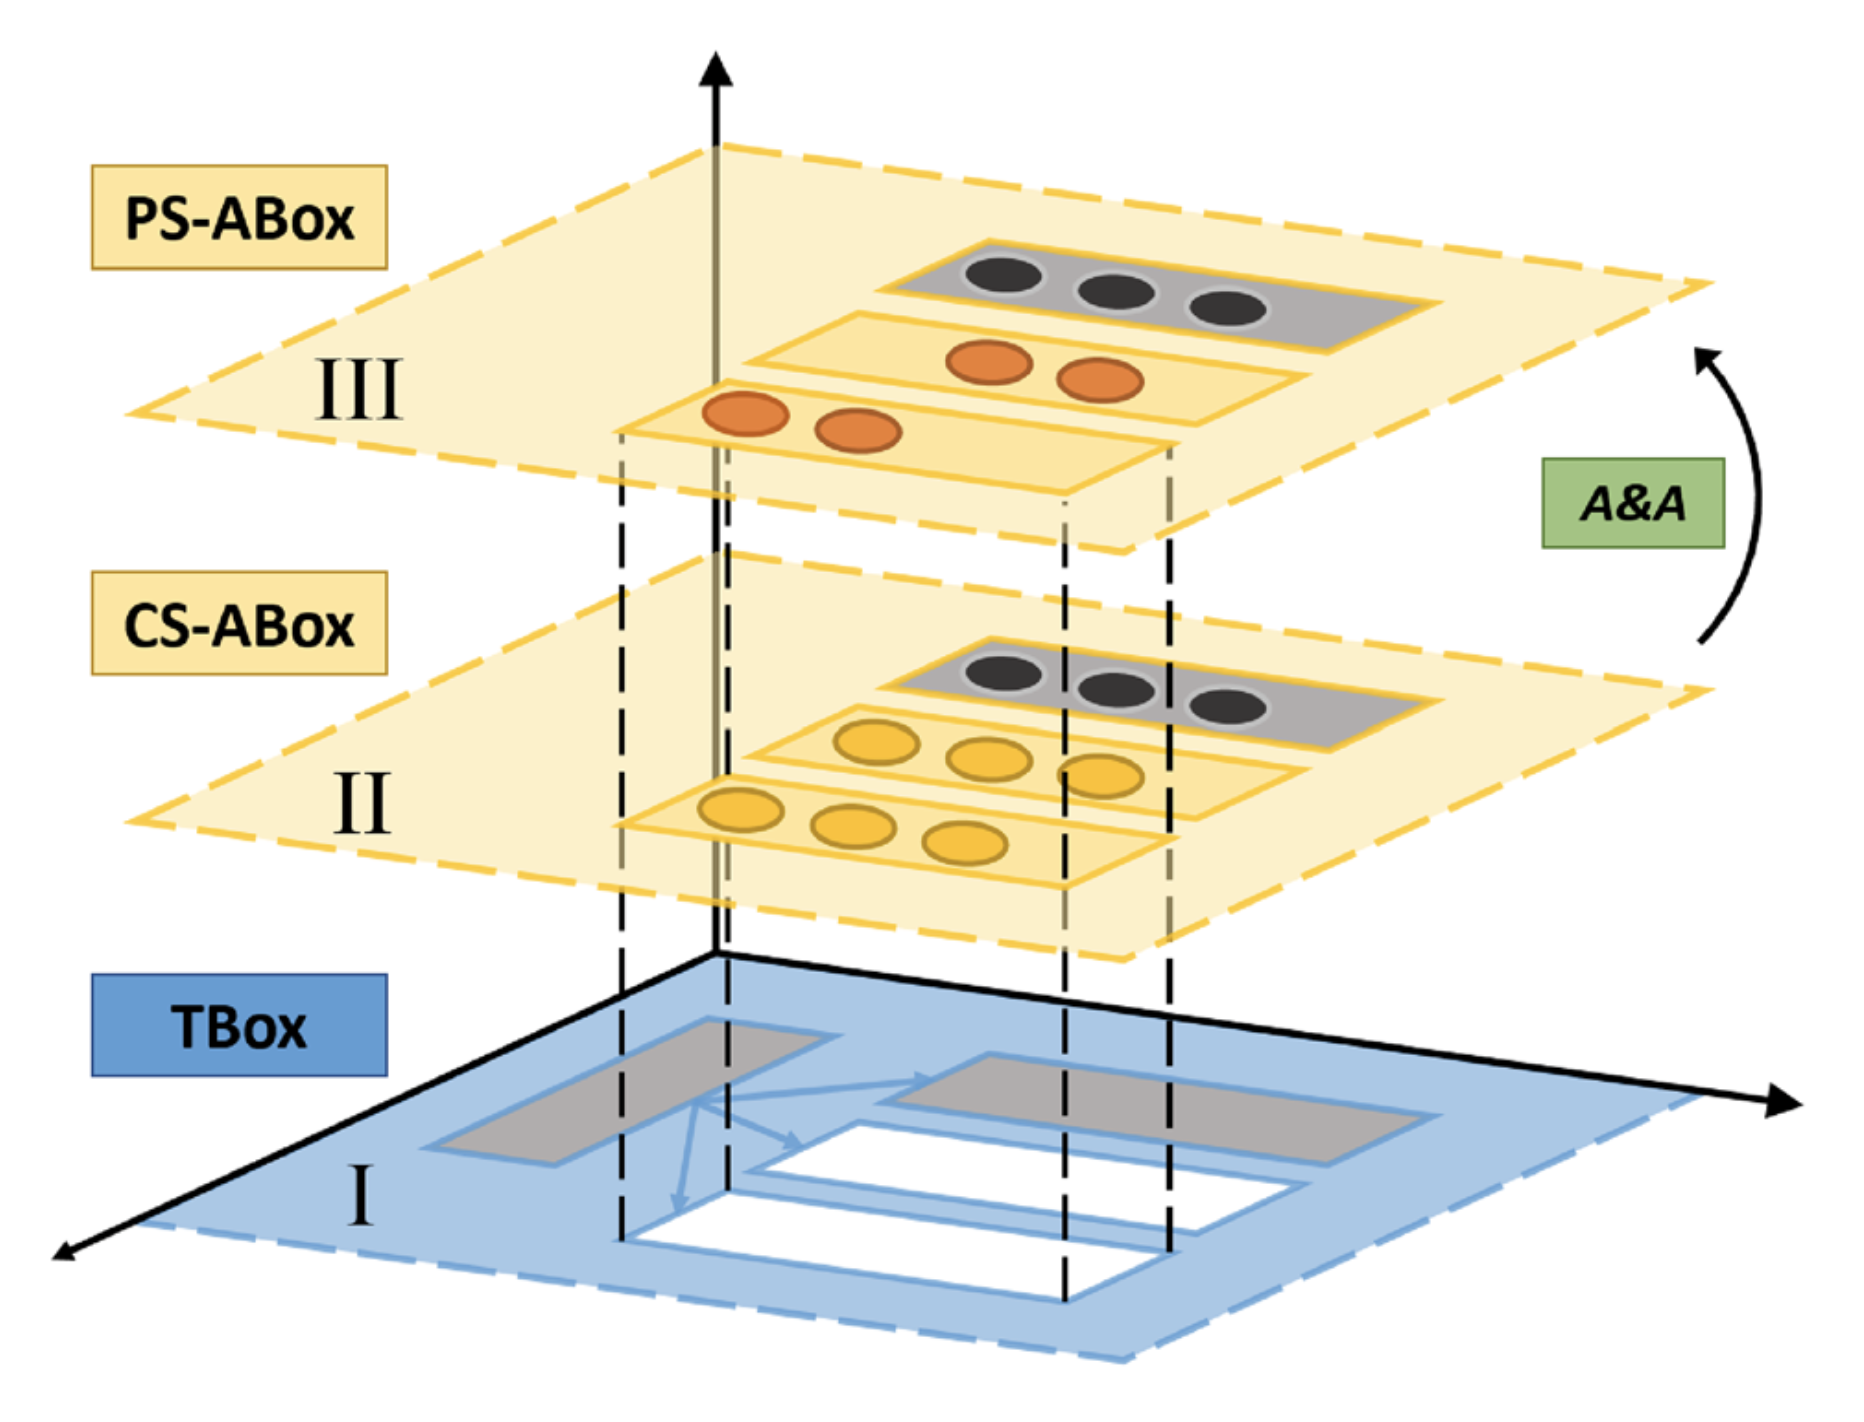
\includegraphics[width=90mm,angle=0]{Knowledge_Representation_Architecture.png}
\end{center}
\vspace{-5mm}
\caption{Knowledge representation architecture for a culturally competent robot. The bottom TBox layer (Layer I) defines the ontology for all knowledge, including domain-specific ontologies and upper ontologies that provide interoperability among domain-specific ontologies  (grey boxes), and ontologies that model cultural-knowledge  (white boxes). The middle CS-ABox layer (Layer II) is the  culture-specific layer which includes instances of national-level cultural knowledge  (yellow circles), as well as instances of knowledge from domain-specific ontologies and upper ontologies (grey circles).  The top PS-ABox layer (Layer III) is the person-specific  layer which includes instances of knowledge about the user (orange circles),  as well as instances of knowledge from domain-specific ontologies and upper ontologies (grey circles). (From Bruno et al. 2019 \cite{Brunoetal2019}.)}
\label{fig:knowledge_representation_architecture}       
\end{figure}


In more detail, the three elements of the knowledge representation architecture are as follows.
\begin{description}
\item [A culture-generic knowledge ontology] is captured in the bottom TBox layer (Layer I). This layer defines the ontology for all knowledge, including domain-specific ontologies and upper ontologies that provide interoperability among domain-specific ontologies  (grey boxes), and ontologies that model cultural-knowledge  (white boxes).  

\item[Culture-specific knowledge] is captured in the middle CS-ABox layer (Layer II). Specifically, this layer  includes instances of national-level cultural knowledge  (yellow circles), as well as instances of knowledge from domain-specific ontologies and upper ontologies.  

\item[Person-specific knowledge] is captured in the top PS-ABox layer (Layer III), including instances of knowledge about the user (orange circles),  as well as instances of knowledge from domain-specific ontologies and upper ontologies
\end{description}
The culture-generic knowledge ontology captures eight types of knowledge, grouped in three categories, as follows.
\begin{enumerate}
\item Context knowledge.
\begin{enumerate}
\item Knowledge about the assisted person.
\item Knowledge about the environment.
\end{enumerate}
\item Robot knowledge.
\begin{enumerate}
\item Knowledge about the actions that the robot can perform.
\item Knowledge about the parameters of these actions.
\item Knowledge about how actions can be combined into higher-level behaviours.
\end{enumerate}
\item Core values knowledge.
\begin{enumerate}
\item Knowledge about the goals of the robot mission.
\item Knowledge about social norms; these can  be considered additional culturally-grounded goals, i.e., constraints  on goals, planning operators, action, and cultural parameters.
\item Knowledge about conversational subject matter.
\end{enumerate}
\end{enumerate}
Here, we are concerned with  2~(a) knowledge about the actions that the robot can perform, 2~(b) knowledge about the parameters of these actions, and  3~(b) knowledge about social norms. The values we use for the action and cultural parameters determine the culturally sensitive nature of the robot's actions. To quote Bruno et al. \cite{Brunoetal2019}:
\begin{quotation}
``Knowledge pertaining to the robot’s sensorimotor and communication capabilities is required by the robot to know what it can do and how the user might prefer it to be done. This knowledge again includes static, {\em a priori} information (e.g., describing the set of commands allowing the robot to perform the Namaste greeting, the associated parameters and their preferable values) and dynamic information (e.g., describing the robot’s current posture and values of related parameters).''
\end{quotation}
These values are then used by the various ROS nodes in the CSSR4Africa system when invoking actions through ROS service requests.  The values themselves are derived from the consensus answers to the survey questions. 

The actions that the robot can perform --- 2~(a) --- depend on the functionality of the system architecture, as described in Deliverable D3.1: animate behaviour, deictic, iconic, and symbolic gesture, overt attention, locomotion and navigation. As such, we do not encode this knowledge explicitly in the CSSR4Africa knowledge base.  Neither do we encode  knowledge about how actions can be combined into higher-level behaviours --- 2~(c) --- explicitly in the CSSR4Africa knowledge base, although some of the knowledge that is revealed and made explicit by the consensus answers to the survey questions does address activities and behaviours.  Thus, the cultural knowledge that is required for the CSSR4Africa project has two forms:
\begin{enumerate}
\item A compendium of culturally sensitive behaviours, activities, actions, and motions.
\item An knowledge ontology to categorize the behaviours, activities, actions, and motions that the Pepper robot can perform.
\item A mapping from the compendium of culturally sensitive behaviours, activities, actions, and motions to the ontology.
\item The action and cultural parameter values  --- 2~(b) and 3~(b) --- that are derived from a subset of the consensus answers.
\end{enumerate}
Item 1 comprises the consensus answers to the fifty-seven questions in the Rwandan cultural knowledge survey documented in Deliverable D1.2. The remaining items are documented in this deliverable.
Note that the mapping from the compendium of culturally sensitive behaviours, activities, actions, and motions to the ontology is partial because there are some behaviours, activities, actions, and motions that the Pepper robot is incapable of performing.




\subsection{A Knowledge Ontology for the Pepper Robot}
%--------------------------------------------
\label{section:pepper}
 

As noted in Section \ref{section:introduction}, Deliverable D1.2 compiles the cultural knowledge required for culturally sensitive human robot interaction between robots and Rwandan people. To be effective, this knowledge must be organized in some manner. This organization is effectively a knowledge ontology that resulted from work carried out early in Task 5.4.1, and documented in this deliverable in Figure \ref{fig:knowledge_ontology}. This ontology was used to guide the preparation of the survey in Deliverable D1.2. As we will see in Section \ref{section:knowledge}, this ontology had to be extended following an analysis of the consensus answers to the questions in the survey.

While Bruno et al. \cite{Brunoetal2019} use the OWL-2 language  to define their ontology, we adopt a simpler approach here that represents the ontology as a tree of concepts, as shown in  Figure \ref{fig:knowledge_ontology}. 
Note that the ontology is restricted to the actions that the Pepper robot can perform.
It explicitly omits forms of non-verbal communication that are important in human-robot interaction, e.g., facial expressions, such as eyebrow and mouth gestures. This provides us with a straightforward way to specify the parameter values for each element in the ontology: we can represent the cultural knowledge with a simple list of key-value pairs, where a key is constructed from the name of a leaf nodes in the ontology tree and the name of its parent.  The values can be either quantitative numeric values or qualitative symbolic values, which can then be interpreted by the ROS node that uses the key-value pair to produce culturally sensistive behaviour.  

\begin{figure}[tbh]
\vspace{-5mm}
\begin{multicols}{2}
\dirtree{%
.1 Cultural Knowledge.
.2 Spatial Interaction.
.2 Verbal Interaction.
.2 Non-verbal Interaction.
}
 
\vspace{5mm}

\dirtree{%
.2 Spatial Interaction.
.3 Standing.
.4 Distance.
.4 Orientation.
.3 Approaching.
.4 Distance.
.4 Orientation.
.4 Velocity.
.3 Passing.
.4 Distance.
.4 Velocity.
.4 Position.
.3 Accompanying.
.4 Distance.
.4 Position.
}

\vspace{5mm}

\dirtree{%
.2 Verbal Interaction.
.3 Expression.
.4 Loudness.
.4 Speed.
.3 Filler.
.4 Sound.
.4 Frequency.
.3 Pause.
.4 Frequency.
.4 Duration.
.3 Turn Taking.
.4 Utterance.
.5 InitiationOrder.
.5 Avoid.
.4 Duration.
}

\columnbreak

\vspace{5mm}

\dirtree{%
.2 Non-verbal Interaction.
.3 Gaze.
.4 Focus of Attention.
.5 Target.
.5 Duration.
.5 Frequency.
.4 Eye Contact.
.5 Duration.
.5 Frequency.
.3 Face or Head Gesture.
.4 Nod.
.5 Extent.
.5 Velocity.
.3 Hand Gesture.
.4 Deictic (Indicating).
.5 Shape.
.5 Duration.
.4 Iconic.
.5 Shape.
.4 Symbolic.
.5 Shape.
.4 Beat During Speech.
.5 Shape.
.5 Intensity.
.5 Frequency.
.3 Body Gesture.
.4 Bow.
.5 Extent.
.5 Velocity.
.4 Sway During Speech.
.5 Intensity.
.5 Frequency.
}
 
\end{multicols}
 
\caption{Original ontology of cultural knowledge. Note that the ontology is restricted to the actions that the Pepper robot can perform.}
\label{fig:knowledge_ontology}       
\end{figure}

\clearpage

 
 

\section{Mapping Rwandan Cultural Knowledge to the Knowledge Ontology Keys}
%===============================================================
\label{section:knowledge}

By itself, an ontology is insufficient, since the knowledge base that is to be used by the robot must be populated by the knowledge that is derived from the survey and documented in Deliverable D1.2.  Thus, we  need to map the knowledge encapsulated in the  consensus answers to each question in the survey to the ontology.  For ease of reference, the survey questions and associated consensus answers in Deliverable D1.2 are reproduced here  in Tables  \ref{table:questions2}  -- \ref{table:AllAnswers3}.  Five of the fifty-seven questions in the cultural knowledge survey  yielded no consensus: 2-4, 2-5,  2-8,   3-28, and 3-30, leaving fifty-two consensus answers to populate the culture knowledge base. This necessitated that the original ontology shown in Figure \ref{fig:knowledge_ontology} be extended to ensure that each item of knowledge has a corresponding entry in the ontology tree. Specifically, if  several survey answers map to a single leaf node in the ontology tree in Fig. \ref{fig:knowledge_ontology}, the ontology was extended by appending suffixes to the leaf labels, e.g., {\small \verb+symbolicShapeRespect+} instead of {\small \verb+symbolicShape+}. This results in an ontology tree with one leaf node for each consensus answer. The onology tree also has several leaf nodes for which there is no associated knowledge, either because no consensus answer emerged, or because no survey question addressed that element of the ontology. The extended ontology is shown in Figures \ref{fig:knowledge_ontology2} and \ref{fig:knowledge_ontology3}.


Table \ref{table:key-value_questions_all} lists the keys  derived from the original ontology tree in Figure \ref{fig:knowledge_ontology}, along with the questions in Parts 2 and 3 of the survey that reveal the associated cultural knowledge listed in Tables  \ref{table:AllAnswers2}  and \ref{table:AllAnswers3}.   
Tables \ref{table:key-value_questions_spatial}  - \ref{table:key-value_questions_nonverbal}  list the keys derived from the extended ontology tree in Figures \ref{fig:knowledge_ontology2} and \ref{fig:knowledge_ontology3}, along with each corresponding question in Parts 2 and 3 of the survey.
 

\begin{table}[H]
\begin{center}
%%\vspace{-10mm}
\begin{tabularx}{\linewidth}{|l|X|}
\hline \hline
 {\small 2-1}   & {\small To show respect, one should lower gaze when greeting someone older.} \vspace{-10mm}\\
 {\small 2-2 }   & {\small  One should suspend work or movements and pay attention when addressed.}\vspace{-10mm}\\
 {\small 2-3 } & {\small  One should keep intermittent eye contact; lack of eye contact depicts disrespect as it shows divided attention during the interaction. }\\
 {\small 2-4 }  & {\small  One should not make persistent eye contact with an older person. }\vspace{-1mm}\\
 {\small 2-5 } & {\small  One should not make eye contact when being corrected by someone. }\vspace{-1mm}\\
 {\small 2-6}   & {\small One should use an open palm of the hand to point to people and objects.}\vspace{-1mm}\\
 {\small 2-7}   & {\small  One should not point an upward facing palm of the hand at someone.}\vspace{-1mm}\\
 {\small 2-8 }    & {\small  One should not use the left hand to point to anything. }\vspace{-1mm}\\
 {\small 2-9 }    & {\small  To show respect, one should bow slightly when greeting someone older.}\vspace{-1mm}\\
 {\small 2-10}    & {\small To show respect, one should raise both hands when greeting.}\\
 {\small 2-11}   & {\small  One should not wave at someone from a distance; one should move towards them to greet them.}\\
 {\small 2-12}  & {\small  One should not use the left hand to hand something to someone.}\\
 {\small 2-13 }   & {\small  To show respect, one should hand over and accept gifts with two hands and do so from the front, facing the recipient.}\\
 {\small 2-14 }   & {\small  To show respect, one should shake hands with the right hand and use the left arm to support the right forearm when doing so.}\\
 {\small 2-15}   & {\small  An appreciation of rhythmic sound and movement is valued. }\\
 {\small 2-16 }   & {\small  To show respect, one should bow slightly and lower gaze when greeting someone older.}\\
 {\small 2-17 }   & {\small  The younger interaction partner should bow when greeting an older person or when rendering a service.}\\
 {\small 2-18 }    & {\small  All interactions should begin with a courteous greeting.}\\
 {\small 2-19 }   & {\small  The younger interaction partner should enable a greeting to be initiated by an older person.}\\
 {\small 2-20 }   & {\small  It is respectful to use local languages and they should be used for verbal interaction when possible. }\\
 {\small 2-21 }   & {\small  One should use formal titles when addressing someone.}\\
 {\small 2-22 }    & {\small  One should engage in a preamble before getting to the point, as being too forward may be regarded as disrespectful.}\\
 {\small 2-23 }   & {\small  One should not interrupt or talk over someone when they are speaking. }\\
 {\small 2-24 }   & {\small  One should not talk loudly to an older person.}\\
 {\small 2-25}   & {\small  Behaviours should focus on fostering social connections and relationships; they should not be purely functional.}\\ 
 {\small 2-26 }    & {\small  One should not walk between two or more people who are conversing because it is considered rude to do so.}\\
 {\small 2-27}   & {\small  One should not walk far ahead of an older person, unless leading the person (in which case, one should walk slightly to the side). }\\
\hline \hline
\end{tabularx}
\end{center}
\caption{Survey questions -- Part 2.  Respondents who took the survey were asked whether these statements were correct or incorrect, or whether they were unsure. }
\label{table:questions2}
\end{table}

\begin{table}[H]
\begin{center}
%%\vspace{-10mm}
\begin{tabularx}{\linewidth}{|l |X|}
\hline \hline
 {\small 3-1 }  & {\small  What distance should you keep when passing someone?}\\
 {\small 3-2 }  & {\small  How should you acknowledge someone when passing them?}\\
 {\small 3-3 }   & {\small  How should you pass a group of two or more people?}\\
 {\small 3-4 }   & {\small  When showing someone older than you the way, where should you position yourself?}\\
 {\small 3-5 }   & {\small  When showing someone the same age as you the way, where should you position yourself?}\\
 {\small 3-6 }   & {\small  When showing someone younger than you the way, where should you position yourself?}\\
 {\small 3-7}   & {\small How should you address someone who is older than you and who you haven't met before?}\\
 {\small 3-8 }   & {\small  How should you address someone who is the same age as you and who you haven't met before?}\\
 {\small 3-9}    & {\small  How should you address someone who is younger than you and who you haven't met before?}\\
 {\small 3-10} & {\small  Should you pause before responding when someone asks you a question? If yes, for how long?}\\
 {\small 3-11 }  & {\small  In an interaction where you and someone else take turns to speak, would you signal that you want to speak? If yes, how do you do that?}\\
 {\small 3-12 }    & {\small  If you are explaining something to someone, what is your primary focus of attention, i.e., where do you direct your gaze?}\\
 {\small 3-13}  & {\small If you are explaining something to someone, how often should you make eye contact?}\\
 {\small 3-14}    & {\small If you are explaining something to someone, how often would you make eye contact if the person was older than you?}\\
 {\small 3-15}    & {\small If you are explaining something to someone, how often would you make eye contact if the person was younger than you?}\\
 {\small 3-16}   & {\small If someone is explaining something to you, what is your primary focus of attention, i.e., where do you direct your gaze?}\\
 {\small 3-17}  & {\small If someone is explaining something to  you,  how often should you make eye contact?}\\
 {\small 3-18}   & {\small If someone is explaining something to  you,  how often would you make eye contact if the person was older than you?}\\
 {\small 3-19}    & {\small If someone is explaining something to you,  how often would you make eye contact if the person was younger than you?}\\	
 {\small 3-20}   & {\small Would you use a face or head gesture to draw someone's attention  to something? If yes, what would that gesture be? }\\
 {\small 3-21}    & {\small Would you use a face, head, hand, or body gesture to express gratitude?}\\
 {\small 3-22 }  & {\small Would you use a face,  head, hand, or body gesture to express agreement?}\\
 {\small 3-23 }    & {\small Would you use a face,  head, hand, or body gesture to express  respect?}\\
 {\small 3-24 }   & {\small Would you use a face,  head, hand, or body gesture to express friendliness?}\\
 {\small 3-25 }    & {\small Would you use a face,  head, hand, or body gesture to express  confusion?}\\
 {\small 3-26 }   & {\small Would you use a face,  head, hand, or body gesture to express comprehension? }\\
 {\small 3-27 }  & {\small Would you use a face,  head, hand, or body gesture to express interest?}\\
 {\small 3-28 }   & {\small Is there  a face head, hand, or body gesture you should not use?}\\
 {\small 3-29 }  & {\small Would you use a hand or body gesture while speaking to someone? }\\
 {\small 3-30 }   & {\small Would you use a hand or body gesture while listening to someone?}\\
\hline \hline
\end{tabularx}
\end{center}
\caption{Survey questions -- Part 3. Respondents who took the survey were given a number of possible answers from which to choose. }
\label{table:questions3}
\end{table}


\begin{table}[H]
\begin{center}
%%\vspace{-5mm}
\begin{tabularx}{\linewidth}{|l |X|}
\hline \hline
 {\small {\bf Question}} & {\small {\bf Consensus Cultural Knowledge}}\\
\hline
{\small 2-1 }  & {\small To show respect, one should lower gaze when greeting someone older.}\\
{\small 2-2 }  & {\small One should suspend work or movements and pay attention when addressed.}\\
{\small 2-3 }  & {\small One should keep intermittent eye contact; lack of eye contact depicts disrespect as it shows divided
attention during the interaction}\\
{\small 2-4 }  & {\small No consensus}\\
{\small 2-5 }  & {\small No consensus}\\
{\small 2-6 }   & {\small One should use an open palm of the hand to point to people and objects.}\\
{\small 2-7 }  & {\small One should not point an upward facing palm of the hand at someone.}\\
{\small 2-8 }  & {\small No consensus}\\
{\small 2-9 }  & {\small To show respect, one should bow slightly when greeting someone older.}\\
{\small 2-10 }  & {\small To show respect, one should raise both hands when greeting.}\\
{\small 2-11 } &  {\small One should not wave at someone from a distance; one should move towards them to greet them}\\
{\small 2-12 }  & {\small One should not use the left hand to hand something to someone}\\
{\small 2-13 } & {\small To show respect, one should hand over and accept gifts with two hands and do so from the front,
facing the recipient}\\
{\small 2-14 }  & {\small To show respect, one should shake hands with the right hand and use the left arm to support the
right forearm when doing so.}\\
{\small 2-15 }  & {\small An appreciation of rhythmic sound and movement is valued.}\\
{\small 2-16 }  & {\small To show respect, one should bow slightly and lower gaze when greeting someone older}\\
{\small 2-17 } & {\small The younger interaction partner should bow when greeting an older person or when rendering a
service}\\
{\small 2-18 }  & {\small All interactions should begin with a courteous greeting.}\\
{\small 2-19 }  & {\small The younger interaction partner should enable a greeting to be initiated by an older person.}\\
{\small 2-20 }  & {\small It is respectful to use local languages and they should be used for verbal interaction when possible.}\\
{\small 2-21 }  & {\small One should use formal titles when addressing someone.}\\
{\small 2-22 }  & {\small One should engage in a preamble before getting to the point, as being too forward may be regarded as disrespectful.}\\
{\small 2-23 }  & {\small One should not interrupt or talk over someone when they are speaking.}\\
{\small 2-24 }  & {\small One should not talk loudly to an older person}\\
{\small 2-25 }  & {\small Behaviours should focus on fostering social connections and relationships; they should not be
purely functional.}\\
{\small 2-26 } & {\small One should not walk between two or more people who are conversing because it is considered
rude to do so.}\\
{\small 2-27 }  & {\small One should not walk far ahead of an older person, unless leading the person (in which case, one
should walk slightly to the side).}\\
\hline \hline
\end{tabularx}
\end{center}
\vspace{-5mm}
\caption{ Consensus answers to the  twenty-seven questions in Part 2 of the cultural knowledge survey. }
\label{table:AllAnswers2}
\end{table}
 
\newpage
\begin{table}[H]
\begin{center}
\vspace{-7mm}
\begin{tabularx}{\linewidth}{|l |X|}
\hline \hline
 {\small {\bf Question}}  & {\small {\bf Consensus Cultural Knowledge}}\\
\hline
\vspace{-0.2mm} {\small 3-1 }   & {\small One should maintain a distance of one meter or less when passing someone.}\\
\vspace{-0.2mm} {\small 3-2 }  & {\small One should say `Hello' or `Muraho' when acknowledging someone while passing them.}\\
\vspace{-0.2mm}  {\small 3-3 }  & {\small One should pass behind a group of two or more people.}\\

\vspace{-0.2mm} {\small 3-4 } & {\small One should position themselves beside someone older when showing them the way.}\\

\vspace{-0.2mm} {\small 3-5 }  & {\small One should position themselves beside someone of the same age when showing them the way.}\\

\vspace{-0.5mm} {\small 3-6 }  & {\small One should position themselves beside someone younger when showing them the way.}\\

\vspace{-0.2mm} {\small 3-7}   & {\small The preferred way to address someone older, and whom you haven't met before, }\\
\vspace{-0.2mm} {\small }   & {\small  is by saying `Muraho' or `Hello'.}\\

\vspace{-0.2mm} {\small 3-8}   & {\small The preferred way to address someone the same age, and whom you haven't met before,  }\\
\vspace{-0.2mm} {\small }   & {\small is by saying  `Muraho' or `Hello'.}\\

\vspace{-0.2mm} {\small 3-9}   & {\small The preferred way to address someone younger, and whom you haven't met before,  }\\
\vspace{-0.2mm} {\small }   & {\small is by saying  `Muraho' or `Hello'.}\\

\vspace{-0.2mm} {\small 3-10 }  & {\small When asked a question, respondents should pause for a few seconds before answering.}\\

\vspace{-0.2mm} {\small 3-11 }   & {\small In turn-based conversations, participants can raise their right hand to signal their desire to speak.}\\

\vspace{-0.2mm} {\small 3-12 }  & {\small When explaining something to someone, you should direct your gaze equally between.}\\
\vspace{-0.2mm} {\small  }  & {\small the person and the object.}\\

\vspace{-0.2mm} {\small 3-13 } & {\small When explaining something to someone, you should make eye contact often.}\\

\vspace{-0.2mm} {\small 3-14 }  & {\small You should make eye contact  often when explaining something to someone older than you.}\\

\vspace{-0.2mm} {\small 3-15 }  & {\small You should make eye contact  often when explaining something to someone younger than you.}\\

\vspace{-0.2mm} {\small 3-16 }  & {\small When someone is explaining something to you, you should direct your gaze equally }\\
\vspace{-0.2mm} {\small }  & {\small   between the person and the object.}\\

\vspace{-0.2mm} {\small 3-17 } & {\small When someone is explaining something to you, you should make eye contact often.}\\

\vspace{-0.2mm} {\small 3-18 }  & {\small If someone is explaining something to you and they are older than you, you should make}\\
\vspace{-0.2mm} {\small  }  & {\small   eye contact  often.}\\


\vspace{-0.2mm} {\small 3-19 }  & {\small If someone is explaining something to you and they are younger than you, you should make }\\ 
\vspace{-0.2mm} {\small  }  & {\small eye contact  often.} \\

\vspace{-0.2mm} {\small 3-20 }  & {\small To draw someone's attention to something, use a head-nodding gesture while looking }\\
\vspace{-0.2mm} {\small  }  & {\small  at the object.}\\

\vspace{-0.2mm} {\small 3-21 }  & {\small To express gratitude, common gestures include nodding, smiling, and bowing the head, }\\
\vspace{-0.2mm} {\small  }  & {\small   using hand gestures like a thumbs up or clasped hands, and slight bowing of the body.}\\

\vspace{-0.2mm} {\small 3-22 }  & {\small To express agreement, common gestures include nodding the head and giving a thumbs up }\\
\vspace{-0.2mm} {\small  }  & {\small  with the right hand.}\\

\vspace{-0.2mm} {\small 3-23 }  & {\small To show respect, common gestures include a slight bow of the head, a greeting or handshake using the right hand supported by the left, and bowing, which is the most frequent body gesture.}\\

\vspace{-0.2mm} {\small 3-24 } & {\small To express friendliness, people commonly use facial gestures like smiling, hand gestures }\\
\vspace{-0.2mm} {\small  } & {\small such as a handshake using both hands or the right hand, and body gestures such as hugging.}\\

\vspace{-0.2mm} {\small 3-25 }  & {\small When expressing confusion, individuals typically use facial gestures like wrinkling or frowning }\\
\vspace{-0.2mm} {\small }  & {\small the brow or tilting the head, hand gestures such as raising both hands or the right hand, }\\
\vspace{-0.2mm} {\small }  & {\small tand body movements that vary according to the situation.}\\

\vspace{-0.2mm} {\small 3-26 }   & {\small When expressing comprehension, individuals typically use head gestures, such as nodding,} \\
\vspace{-0.2mm} {\small  }   & {\small hand gestures like a right-hand thumbs-up, and body gestures that vary by situation.} \\

\vspace{-0.2mm} {\small 3-27 } & {\small When expressing interest, nodding and smiling are the most common gestures.} \\
\vspace{-0.2mm} {\small } & {\small Hand gestures, such as giving a thumbs up with the right hand, and body gestures such as} \\
\vspace{-0.2mm} {\small } & {\small  facing someone, are used less frequently.} \\

\vspace{-0.2mm} {\small 3-28 } & {\small No consensus.} \\

\vspace{-0.2mm} {\small 3-29 }  & {\small One should use various body and hand gestures while speaking to someone. } \\
\vspace{-0.2mm}  & {\small The most recommended gestures are slight body movement and slightly moving both hands.} \\

\vspace{-0.2mm} {\small 3-30 } & {\small No consensus.} \\
\hline \hline
\end{tabularx}
\end{center}
\vspace{-5mm}
\caption{ Consensus answers to the thirty questions in Part 3 of the cultural knowledge survey.}
\label{table:AllAnswers3}
\end{table}



\begin{table}[H]
\begin{center}
%%\vspace{-10mm}
\begin{tabular}{|l l|}
\hline \hline
 {\small \bf Key  }                                         &  {\small \bf Questions }      \\
\hline \hline
\multicolumn{2}{|c|}{{\footnotesize \bf Spatial Interaction}} \\
\hline
{\footnotesize \verb+standingDistance+} 	           &{\footnotesize \verb++} \vspace{-1mm}\\
{\footnotesize \verb+standingOrientation+} 	           &  {\footnotesize \verb++} \vspace{-1mm}\\
{\footnotesize \verb+approachingDistance+} 	   &  {\footnotesize \verb++} \vspace{-1mm}\\
{\footnotesize \verb+approachingOrientation+} 	   & {\footnotesize \verb++} \vspace{-1mm}\\
{\footnotesize \verb+approachingVelocity+} 	           & {\footnotesize \verb++} \vspace{-1mm}\\
{\footnotesize \verb+passingDistance+} 	           &{\footnotesize 3-1} \vspace{-1mm}\\
{\footnotesize \verb+passingVelocity+} 	                  & {\footnotesize \verb++} \vspace{-1mm}\\
{\footnotesize \verb+passingPosition+} 	           & {\footnotesize 2-26, 3-3} \vspace{-1mm}\\
{\footnotesize \verb+accompanyingDistance+} 	   & {\footnotesize 2-27, 3-4, 3-5, 3-6} \vspace{-1mm}\\
{\footnotesize \verb+accompanyingPosition+} 	   & {\footnotesize \verb++} \\
\hline \hline


\multicolumn{2}{|c|}{{\footnotesize \bf Verbal Interaction}} \\
\hline
{\footnotesize \verb+expressionLoudness+} 	           & {\footnotesize 2-24} \vspace{-1mm}\\
%%{\footnotesize \verb+expressionPhrase+} 	           & {\footnotesize 2-15, 2-18, 2-20, 2-21, 2-22, 2-25, 3-2, 3-7, 3-8, 3-9} \vspace{-1mm}\\
{\footnotesize \verb+expressionSpeed+} 	            & {\footnotesize \verb++} \vspace{-1mm}\\
{\footnotesize \verb+fillerSound+} 	                   & {\footnotesize \verb++} \vspace{-1mm}\\
{\footnotesize \verb+fillerFrequency+} 	                   & {\footnotesize \verb++} \vspace{-1mm}\\
{\footnotesize \verb+pauseFrequency+} 	           & {\footnotesize \verb++} \vspace{-1mm}\\
{\footnotesize \verb+pauseDuration+} 	                    & {\footnotesize 3-10 }\vspace{-1mm} \\
{\footnotesize \verb+turnTakingUtterance+}            & {\footnotesize 2-19, 2-23 } \vspace{-1mm}\\
{\footnotesize \verb+turnTakingDuration+} 	            & {\footnotesize \verb++}\\
\hline \hline


\multicolumn{2}{|c|}{{\footnotesize \bf Non-Verbal Interraction}} \\
\hline
\multicolumn{2}{|c|}{{\footnotesize Gaze}} \\
\hline
{\footnotesize \verb+focusofAttentionTarget+} 	    & {\footnotesize 2-1, 2-2, 2-16, 3-12, 3-16} \vspace{-1mm}\\
{\footnotesize \verb+focusofAttentionDuration+}     & {\footnotesize \verb++} \vspace{-1mm}\\
{\footnotesize \verb+focusofAttentionFrequency+}   & {\footnotesize \verb++} \vspace{-1mm}\\
{\footnotesize \verb+eyeContactDuration+} 	            & {\footnotesize 2-3, 2-4, 2-5, 3-2 } \vspace{-1mm}\\
{\footnotesize \verb+eyeContactFrequency+} 	    & {\footnotesize 3-13, 3-14, 3-15, 3-17, 3-18, 3-19 } \\
\hline
\multicolumn{2}{|c|}{{\footnotesize Face or Head Gesture}} \\
\hline
{\footnotesize \verb+nodExtent+} 	                           & {\footnotesize 3-20, 3-21, 3-22, 3-23, 3-24, 3-26, 3-27 }\vspace{-1mm} \\
{\footnotesize \verb+nodVelocity+} 	                   & {\footnotesize  }\\
\hline
\multicolumn{2}{|c|}{{\footnotesize Hand Gesture}} \\
\hline
{\footnotesize \verb+deicticShape+} 	                 & {\footnotesize 2-6, 2-7, 2-8 } \vspace{-1mm}\\
%%{\footnotesize \verb+deicticRestriction+} 	          & {\footnotesize 2-7, 2-8 } \vspace{-1mm}\\
{\footnotesize \verb+deicticDuration+} 	                 & {\footnotesize \verb++} \vspace{-1mm}\\
{\footnotesize \verb+iconicShape+} 	                 & {\footnotesize 3-29, 3-30  } \vspace{-1mm}\\
{\footnotesize \verb+symbolicShape+} 	                 & {\footnotesize 2-10, 2-13, 2-14, 3-11, 3-21, 3-22, 3-23, 3-24, 3-25, 3-26, 3-27  }\vspace{-1mm} \\
%%{\footnotesize \verb+symbolicRestriction+} 	  & {\footnotesize 2-11, 2-12  }\vspace{-1mm} \\
{\footnotesize \verb+beatShape+} 	                         & {\footnotesize \verb++}\vspace{-1mm} \\
{\footnotesize \verb+beatIntensity+} 	                 & {\footnotesize \verb++} \vspace{-1mm}\\
{\footnotesize \verb+beatFrequency+} 	                 & {\footnotesize \verb++} \\
\hline
\multicolumn{2}{|c|}{{\footnotesize Body Gesture}} \\
\hline
{\footnotesize \verb+bowExtent+} 	                        & {\footnotesize 2-9, 2-16, 2-17, 3-21, 3-22, 3-23, 3-24, 3-26, 3-27} \vspace{-1mm}\\
{\footnotesize \verb+bowVelocity+}                       & {\footnotesize \verb++} \vspace{-1mm}\\
{\footnotesize \verb+swayIntensity+} 	                & {\footnotesize 3-21, 3-22, 3-23, 3-24, 3-25, 3-26, 3-27} \vspace{-1mm}\\
{\footnotesize \verb+swayFrequency+} 	                & {\footnotesize \verb++} \\
\hline \hline
\end{tabular}
\end{center}
\caption{Keys for specifying culturally sensitive actions and the corresponding questions in Parts 2 and 3 of the survey that reveal the associated cultural knowledge, prior to extending the ontology, i.e., using the ontology depicted in Fig. \ref{fig:knowledge_ontology}.}
\label{table:key-value_questions_all}
\end{table}

 

\begin{figure}[H]
\vspace{-8mm}
\begin{multicols}{3}
\dirtree{%
.1 Cultural Knowledge.
.2 Spatial Interaction.
.2 Verbal Interaction.
.2 Non-verbal Interaction.
}

\vspace{3mm}
\dirtree{%
.2 Spatial Interaction.
.3 Standing.
.4 Distance.
.4 Orientation.
.3 Approaching.
.4 Distance.
.4 Orientation.
.4 Velocity.
.3 Passing.
.4 Distance.
.4 Velocity.
.4 Position.
.5 Preferred.
.5 Avoid.
.3 Accompanying.
.4 Distance.
.5 Leading.
.4 Position.
.5 Leading.
.5 Older.
.5 Same\,Age.
.5 Younger.
}


\columnbreak
~
\vspace{17mm}

\dirtree{%
.2 Verbal Interaction.
.3 Expression.
.4 Loudness.
.4 Speed.
.4 Phrase.
.5 Language.
.5 Rhythm.
.6 English.
.6 isiZulu.
.6 Kinyarwanda.
.5 Greeting.
.6 English.
.6 isiZulu.
.6 Kinyarwanda.
.5 Title.
.6 English.
.6 isiZulu.
.6 Kinyarwanda.
.5 Preamble.
.6 English.
.6 isiZulu.
.6 Kinyarwanda.
.5 Social.
.6 English.
.6 isiZulu.
.6 Kinyarwanda.
.5 Address\,Older.
.6 English.
.6 isiZulu.
.6 Kinyarwanda.
.5 Address\,Same\,Age.
.6 English.
.6 isiZulu.
.6 Kinyarwanda.
.5 Address\,Younger.
.6 English.
.6 isiZulu.
.6 Kinyarwanda.
.5 Passing.
.6 English.
.6 isiZulu.
.6 Kinyarwanda.
}


\columnbreak
~
\vspace{19mm}
\dirtree{%
.2 ~~~.
.3 Filler.
.4 Sound.
.4 Frequency.
.3 Pause.
.4 Frequency.
.4 Duration.
.3 Turn Taking.
.4 Utterance.
.6 English.
.6 isiZulu.
.6 Kinyarwanda.
.4 Duration.
.4 Initiation\,Order.
.4 Avoid.
}
\end{multicols}
\vspace{-5mm}
\caption{Extended ontology of cultural knowledge  after mapping Rwandan cultural knowledge to the knowledge ontology.}
\label{fig:knowledge_ontology2}       
\end{figure}
 



\begin{figure}[H]
%%\vspace{-5mm}
\begin{multicols}{2}

~
\vspace{9.5mm}

\dirtree{%
.2 Non-verbal Interaction.
.3 Gaze.
.4 Focus of Attention.
.5 Target.
.6 Respect.
.6 Addressed.
.6 Explanation\,To.
.6 Explanation\,By.
.5 Duration.
.5 Frequency.
.4 Eye Contact.
.5 Duration.
.5 Frequency.
.6 Explaining\,To.
.6 Explaining\,To\,Older.
.6 Explaining\,To\,Younger.
.6 Explaining\,By.
.6 Explaining\,By\,Older.
.6 Explaining\,By\,Younger.
.3 Face or Head Gesture.
.4 Nod.
.5 Extent.
.6 Attention.
.6 Gratitude.
.6 Agreement.
.6 Respect.
.6 Friendliness.
.6 Comprehension.
.6 Interest.
.5 Velocity.
}

\columnbreak
~
\vspace{9.5mm}
\dirtree{%
.2 ~~~. 
.3 Hand Gesture.
.4 Deictic.
.5 Shape.
.5 Duration.
.5 Avoid.
.4 Iconic.
.5 Shape.
.4 Symbolic.
.5 Shape.
.6 Respect.
.6 Turn Taking.
.6 Gratitude.
.6 Agreement.
.6 Friendliness.
.6 Confusion.
.6 Comprehension.
.6 Interest.
.6 Handover.
.6 Handshake.
.5 Avoid.
.6 Wave.
.6 Handover.
.4 Beat During Speech.
.5 Shape.
.5 Intensity.
.5 Frequency.
.3 Body Gesture.
.4 Bow.
.5 Extent.
.6 Greeting.
.6 Respect.
.6 Gratitude.
.5 Velocity.
.4 Sway~During~Speech.
.5 Intensity.
.5 Frequency.
}
\end{multicols}

\caption{Extended ontology of cultural knowledge  after mapping Rwandan cultural knowledge to the knowledge ontology.}
\label{fig:knowledge_ontology3}       
\end{figure}

 


\begin{table}[H]
\begin{center}
\begin{tabular}{|l l|}
\hline \hline
\multicolumn{2}{|c|}{{\small \bf Spatial Interaction}} \\
\hline \hline
 {\small Key  }                                         &  {\small  Questions }      \\
\hline
{\footnotesize \verb+standingDistance+} 	           &{\footnotesize \verb++} \vspace{-1mm}\\
{\footnotesize \verb+standingOrientation+} 	           &  {\footnotesize \verb++} \vspace{-1mm}\\
{\footnotesize \verb+approachingDistance+} 	   &  {\footnotesize \verb++} \vspace{-1mm}\\
{\footnotesize \verb+approachingOrientation+} 	   & {\footnotesize \verb++} \vspace{-1mm}\\
{\footnotesize \verb+approachingVelocity+} 	           & {\footnotesize \verb++} \vspace{-1mm}\\
{\footnotesize \verb+passingDistance+} 	           &{\footnotesize 3-1} \vspace{-1mm}\\
{\footnotesize \verb+passingVelocity+} 	                  & {\footnotesize \verb++} \vspace{-1mm}\\
{\footnotesize \verb+passingPositionPreferred+} 	    & {\footnotesize 2-26} \vspace{-1mm}\\
{\footnotesize \verb+passingPositionAvoid+} 	    & {\footnotesize 3-3} \vspace{-1mm}\\
{\footnotesize \verb+accompanyingDistanceLeading+} 	   & {\footnotesize 2-27} \vspace{-1mm}\\
{\footnotesize \verb+accompanyingPositionLeading+} 	         & {\footnotesize 2-27 \verb++} \vspace{-1mm}\\
{\footnotesize \verb+accompanyingPositionOlder+} 	         & {\footnotesize 3-4\verb++} \vspace{-1mm}\\
{\footnotesize \verb+accompanyingPositionSameAge+} 	   & {\footnotesize 3-5\verb++} \vspace{-1mm}\\
{\footnotesize \verb+accompanyingPositionYounger+} 	   & {\footnotesize 3-6\verb++}\\
\hline \hline
\end{tabular}
\end{center}
\caption{Keys for specifying culturally sensitive spatial interaction and the corresponding questions in Parts 2 and 3 of the survey that reveal the associated cultural knowledge, after extending the ontology, i.e., using the ontology depicted in Figs. \ref{fig:knowledge_ontology2} and \ref{fig:knowledge_ontology3}.}
\label{table:key-value_questions_spatial}
\end{table}

\begin{table}[H]
\begin{center}
\begin{tabular}{|l l|}
\hline \hline
\multicolumn{2}{|c|}{{\small \bf Verbal Interaction}} \\
\hline \hline
 {\small  Key  }                                         &  {\small Questions }      \\
\hline
{\footnotesize \verb+expressionLoudness+} 	           & {\footnotesize 2-24} \vspace{-1mm}\\
{\footnotesize \verb+expressionSpeed+} 	            & {\footnotesize \verb++} \vspace{-1mm}\\
{\footnotesize \verb+phraseLanguage+} 	           & {\footnotesize 2-20} \vspace{-1mm}\\
{\footnotesize \verb+phraseRhythmEnglish+} 	           & {\footnotesize 2-15 } \vspace{-1mm}\\
{\footnotesize \verb+phraseRhythmIsiZulu+} 	           & {\footnotesize 2-15 } \vspace{-1mm}\\
{\footnotesize \verb+phraseRhythmKinyarwanda+} 	           & {\footnotesize 2-15 } \vspace{-1mm}\\
{\footnotesize \verb+phraseGreetingEnglish+} 	           & {\footnotesize  2-18} \vspace{-1mm}\\
{\footnotesize \verb+phraseGreetingIsiZulu+} 	           & {\footnotesize  2-18} \vspace{-1mm}\\
{\footnotesize \verb+phraseGreetingKinyarwanda+} 	           & {\footnotesize  2-18} \vspace{-1mm}\\
{\footnotesize \verb+phraseTitleEnglish+} 	           & {\footnotesize 2-21} \vspace{-1mm}\\
{\footnotesize \verb+phraseTitleIsiZulu+} 	           & {\footnotesize 2-21} \vspace{-1mm}\\
{\footnotesize \verb+phraseTitleKinyarwanda+} 	           & {\footnotesize 2-21} \vspace{-1mm}\\
{\footnotesize \verb+phrasePreambleEnglish+} 	           & {\footnotesize 2-22 } \vspace{-1mm}\\
{\footnotesize \verb+phrasePreambleIsiZulu+} 	           & {\footnotesize 2-22 } \vspace{-1mm}\\
{\footnotesize \verb+phrasePreambleKinyarwanda+} 	           & {\footnotesize 2-22 } \vspace{-1mm}\\
{\footnotesize \verb+phraseSocialEnglish+} 	           & {\footnotesize  2-25} \vspace{-1mm}\\
{\footnotesize \verb+phraseSocialIsiZulu+} 	           & {\footnotesize  2-25} \vspace{-1mm}\\
{\footnotesize \verb+phraseSocialKinyarwanda+} 	           & {\footnotesize  2-25} \vspace{-1mm}\\
{\footnotesize \verb+phraseAddressOlderEnglish+} 	           & {\footnotesize  3-7} \vspace{-1mm}\\
{\footnotesize \verb+phraseAddressOlderIsiZulu+} 	           & {\footnotesize  3-7} \vspace{-1mm}\\
{\footnotesize \verb+phraseAddressOlderKinyarwanda+} 	           & {\footnotesize  3-7} \vspace{-1mm}\\
{\footnotesize \verb+phraseAddressSameAgeEnglish+} 	           & {\footnotesize 3-8} \vspace{-1mm}\\
{\footnotesize \verb+phraseAddressSameAgeIsiZulu+} 	           & {\footnotesize 3-8} \vspace{-1mm}\\
{\footnotesize \verb+phraseAddressSameAgeKinyarwanda+} 	           & {\footnotesize 3-8} \vspace{-1mm}\\
{\footnotesize \verb+PhraseAddressYoungerEnglish+} 	           & {\footnotesize 3-9} \vspace{-1mm}\\
{\footnotesize \verb+PhraseAddressYoungerIsiZulu+} 	           & {\footnotesize 3-9} \vspace{-1mm}\\
{\footnotesize \verb+PhraseAddressYoungerKinyarwanda+} 	           & {\footnotesize 3-9} \vspace{-1mm}\\
{\footnotesize \verb+PhrasePassingEnglish+} 	           & {\footnotesize  3-2 } \vspace{-1mm}\\
{\footnotesize \verb+PhrasePassingIsiZulu+} 	           & {\footnotesize  3-2 } \vspace{-1mm}\\
{\footnotesize \verb+PhrasePassingKinyarwanda+} 	           & {\footnotesize  3-2 } \vspace{-1mm}\\
{\footnotesize \verb+fillerSound+} 	                   & {\footnotesize \verb++} \vspace{-1mm}\\
{\footnotesize \verb+fillerFrequency+} 	                   & {\footnotesize \verb++} \vspace{-1mm}\\
{\footnotesize \verb+pauseFrequency+} 	           & {\footnotesize \verb++} \vspace{-1mm}\\
{\footnotesize \verb+pauseDuration+} 	                    & {\footnotesize 3-10 }\vspace{-1mm} \\
{\footnotesize \verb+turnTakingUtteranceEnglish+} 	            & {\footnotesize \verb++}\vspace{-1mm}\\
{\footnotesize \verb+turnTakingUtteranceIsiZulu+} 	            & {\footnotesize \verb++}\vspace{-1mm}\\
{\footnotesize \verb+turnTakingUtteranceKinyarwanda+} 	            & {\footnotesize \verb++}\vspace{-1mm}\\
{\footnotesize \verb+turnTakingDuration+} 	            & {\footnotesize \verb++}\vspace{-1mm}\\
{\footnotesize \verb+turnTakingInitiationOrder+}            & {\footnotesize 2-19 } \vspace{-1mm}\\
{\footnotesize \verb+turnTakingAvoid+}            & {\footnotesize 2-23 } \\
\hline \hline
\end{tabular}
\end{center}
\caption{Keys for specifying culturally sensitive verbal interaction and the corresponding questions in Parts 2 and 3 of the survey that reveal the associated cultural knowledge, after extending the ontology, i.e., using the ontology depicted in Figs. \ref{fig:knowledge_ontology2} and \ref{fig:knowledge_ontology3}.}
\label{table:key-value_questions_verbal}
\end{table}


\begin{table}[H]
\vspace{-10mm}
\begin{center}
\begin{tabular}{|l l|}
\hline \hline
\multicolumn{2}{|c|}{{\small \bf Non-verbal Interaction}} \\
\hline \hline
 {\small Key  }                                         &  {\small Questions }      \\
\hline
\multicolumn{2}{|c|}{{\footnotesize Gaze}} \\
\hline
{\footnotesize \verb+focusofAttentionTargetRespect+} 	    & {\footnotesize 2-1, 2-16} \vspace{-1.01mm}\\
{\footnotesize \verb+focusofAttentionTargetAddressed+} 	    & {\footnotesize 2-2} \vspace{-1.01mm}\\
{\footnotesize \verb+focusofAttentionTargetExplanationTo+} 	    & {\footnotesize 3-12} \vspace{-1.01mm}\\
{\footnotesize \verb+focusofAttentionTargetExplanationBy+} 	    & {\footnotesize 3-16} \vspace{-1.01mm}\\
{\footnotesize \verb+focusofAttentionDuration+}     & {\footnotesize \verb++} \vspace{-1.01mm}\\
{\footnotesize \verb+focusofAttentionFrequency+}   & {\footnotesize \verb++} \vspace{-1.01mm}\\
{\footnotesize \verb+eyeContactDuration+} 	            & {\footnotesize 2-3 } \vspace{-1mm}\\
{\footnotesize \verb+eyeContactFrequencyExplainingTo+} 	                   & {\footnotesize 3-13 } \vspace{-1.01mm}\\
{\footnotesize \verb+eyeContactFrequencyExplainingToOlder+} 	           & {\footnotesize 3-14} \vspace{-1.01mm}\\
{\footnotesize \verb+eyeContactFrequencyExplainingToYounger+} 	    & {\footnotesize 3-15 }\vspace{-1.01mm} \\
{\footnotesize \verb+eyeContactFrequencyExplainingBy+} 	                   & {\footnotesize 3-17 } \vspace{-1.01mm}\\
{\footnotesize \verb+eyeContactFrequencyExplainingByOlder+}     	    & {\footnotesize 3-18} \vspace{-1.01mm}\\
{\footnotesize \verb+eyeContactFrequencyExplainingByYounger+} 	    & {\footnotesize 3-19 }\\
\hline
\multicolumn{2}{|c|}{{\footnotesize Face or Head Gesture}} \\
\hline
{\footnotesize \verb+nodExtentAttention+} 	                           & {\footnotesize 3-20 }\vspace{-1.01mm} \\
{\footnotesize \verb+nodExtentGratitude+} 	                           & {\footnotesize 3-21}\vspace{-1.01mm} \\
{\footnotesize \verb+nodExtentAgreement+} 	                           & {\footnotesize   3-22 }\vspace{-1.01mm} \\
{\footnotesize \verb+nodExtentRespect+} 	                           & {\footnotesize   3-23}\vspace{-1.01mm} \\
{\footnotesize \verb+nodExtentFriendliness+} 	                           & {\footnotesize 3-24 }\vspace{-1.01mm} \\
{\footnotesize \verb+nodExtentComprehension+} 	                           & {\footnotesize 3-26}\vspace{-1.01mm} \\
{\footnotesize \verb+nodExtentInterest+} 	                           & {\footnotesize  3-27 }\vspace{-1.01mm} \\
{\footnotesize \verb+nodVelocity+} 	                   & {\footnotesize  }\\
\hline
\multicolumn{2}{|c|}{{\footnotesize Hand Gesture}} \\
\hline
{\footnotesize \verb+deicticShape+} 	                 & {\footnotesize 2-6} \vspace{-1.01mm}\\
{\footnotesize \verb+deicticDuration+} 	                 & {\footnotesize \verb++} \vspace{-1.01mm}\\
{\footnotesize \verb+deicticAvoid+} 	          & {\footnotesize 2-7} \vspace{-1.01mm}\\
{\footnotesize \verb+iconicShape+} 	                 & {\footnotesize 3-29} \vspace{-1.01mm}\\
{\footnotesize \verb+symbolicShapeRespect+} 	                 & {\footnotesize 2-10, 3-23 }\vspace{-1.01mm} \\
{\footnotesize \verb+symbolicShapeTurnTaking+} 	                 & {\footnotesize 3-11  }\vspace{-1.01mm} \\
{\footnotesize \verb+symbolicShapeGratitude+} 	                 & {\footnotesize 3-21 }\vspace{-1.01mm} \\
{\footnotesize \verb+symbolicShapeAgreement+} 	                 & {\footnotesize 3-22 }\vspace{-1.01mm} \\
{\footnotesize \verb+symbolicShapeFriendliness+} 	                 & {\footnotesize 3-24 }\vspace{-1.01mm} \\
{\footnotesize \verb+symbolicShapeConfusion+} 	                 & {\footnotesize  3-25}\vspace{-1.01mm} \\
{\footnotesize \verb+symbolicShapeComprehension+} 	                 & {\footnotesize 3-26 }\vspace{-1.01mm} \\
{\footnotesize \verb+symbolicShapeInterest+} 	                 & {\footnotesize 3-27 }\vspace{-1.01mm} \\
{\footnotesize \verb+symbolicShapeHandover+} 	                 & {\footnotesize  2-13}\vspace{-1.01mm} \\
{\footnotesize \verb+symbolicShapeHandshake+} 	                 & {\footnotesize   2-14  }\vspace{-1.01mm} \\
{\footnotesize \verb+symbolicAvoidWave+} 	  & {\footnotesize 2-11 }\vspace{-1.01mm} \\
{\footnotesize \verb+symbolicAvoidHandover+} 	  & {\footnotesize 2-12  }\vspace{-1.01mm} \\
{\footnotesize \verb+beatShape+} 	                         & {\footnotesize \verb++}\vspace{-1.01mm} \\
{\footnotesize \verb+beatIntensity+} 	                 & {\footnotesize \verb++} \vspace{-1.01mm}\\
{\footnotesize \verb+beatFrequency+} 	                 & {\footnotesize \verb++} \\
\hline
\multicolumn{2}{|c|}{{\footnotesize Body Gesture}} \\
\hline
{\footnotesize \verb+bowExtentGreeting+} 	                        & {\footnotesize 2-9} \vspace{-1.01mm}\\
{\footnotesize \verb+bowExtentRespect+} 	                        & {\footnotesize 2-16, 2-17, 3-23} \vspace{-1.01mm}\\
{\footnotesize \verb+bowExtentGratitude+} 	                        & {\footnotesize  3-21} \vspace{-1.01mm}\\
{\footnotesize \verb+bowVelocity+}                       & {\footnotesize  } \vspace{-1.01mm}\\
{\footnotesize \verb+swayIntensity+} 	                & {\footnotesize  } \vspace{-1.01mm}\\
{\footnotesize \verb+swayFrequency+} 	                & {\footnotesize 3-29} \\
\hline \hline
\end{tabular}
\end{center}
\vspace{-6mm}
\caption{Keys for specifying culturally sensitive non-verbal interaction and the corresponding questions in Parts 2 and 3 of the survey that reveal the associated cultural knowledge, after extending the ontology, i.e., using the ontology depicted in Figs. \ref{fig:knowledge_ontology2} and \ref{fig:knowledge_ontology3}.}
\label{table:key-value_questions_nonverbal}
\end{table}



\section{Culture Knowledge Base}
%=====================
\label{section:knowledge_base}

Tables \ref{table:key-knowledge_pairs1}--\ref{table:key-knowledge_pairs3}  lists the knowledge associated with each key in the extended ontology tree: spatial interaction, verbal interaction, and non-verbal interaction.

Tables \ref{table:key-value_pairs1} --\ref{table:key-value_pairs3} list the key-value pairs, i.e., with numeric or symbolic values that encapsulate the cultural knowledge.  These numeric or symbolic values can then be used directly in the robot mission interpreter, i.e., the {\small \tt behaviorController} ROS node, and passed as arguments in the service requests it issues to the nodes in the system architecture to achieve culturally sensitive behavior.

The robot may need to say other phrases to prompt the user, reply to the user, or just ensure flow in the dialogue. These were not captured in the cultural knowledge survey but they are necessary, nonetheless.  We include them here as  a set of utility verbal interaction phrases; see Table \ref{table:key-value_pairs4}.

The key-value pairs are stored in a file {\tt \small cultureKnowledgeBaseInput.dat}. This file is read and the value-pairs are accessed using a helper class {\tt \small CultureKnowledgeBase} described in Section~\ref{section:implementation}.  


\begin{table}[H]
\begin{center}
%%\vspace{-10mm}
\begin{tabular}{|l l|}
\hline \hline
\multicolumn{2}{|c|}{{\small \bf Spatial Interaction}} \\
\hline \hline
 {\small Key  }                                         &  {\small Values }      \\
\hline
{\footnotesize \verb+standingDistance+} 	           & {\footnotesize \verb++ } \vspace{-1mm}\\
{\footnotesize \verb+standingOrientation+} 	           & {\footnotesize \verb++} \vspace{-1mm}\\
{\footnotesize \verb+approachingDistance+} 	   & {\footnotesize \verb++} \vspace{-1mm}\\
{\footnotesize \verb+approachingOrientation+} 	   & {\footnotesize \verb++} \vspace{-1mm}\\
{\footnotesize \verb+approachingVelocity+} 	           & {\footnotesize \verb++} \vspace{-1mm}\\
{\footnotesize \verb+passingDistance+} 	           & {\footnotesize \verb++ 1m or less} \vspace{-1mm}\\
{\footnotesize \verb+passingVelocity+} 	                  & {\footnotesize \verb++  } \vspace{-1mm}\\
{\footnotesize \verb+passingPositionPreferred+} 	  & {\footnotesize \verb++ Pass behind a group of two or more people} \vspace{-1mm}\\
{\footnotesize \verb+passingPositionAvoid+}          & {\footnotesize \verb++ Walk between two or more people who are conversing} \vspace{-1mm}\\ 
{\footnotesize \verb+accompanyingDistanceLeading+}  & {\footnotesize \verb++ Do not walk far ahead of an older person} \vspace{-1mm}\\
{\footnotesize \verb+accompanyingPositionLeading+} 	   & {\footnotesize \verb++ Walk slightly ahead and to the side} \vspace{-1mm}\\
{\footnotesize \verb+accompanyingPositionOlder+} 	   & {\footnotesize \verb++ Walk to the side} \vspace{-1mm}\\
{\footnotesize \verb+accompanyingPositionSameAge+}  & {\footnotesize \verb++ Walk to the side} \vspace{-1mm}\\
{\footnotesize \verb+accompanyingPositionYounger+}  & {\footnotesize \verb++ Walk to the side} \\
\hline \hline
\end{tabular}
\end{center}
\caption{Spatial interaction: key-knowledge pairs for specifying culturally sensitive actions after extending the ontology, i.e., using the ontology depicted in Figs. \ref{fig:knowledge_ontology2} and \ref{fig:knowledge_ontology3}.}
\label{table:key-knowledge_pairs1}
\end{table}

 
\begin{table}[H]
\begin{center}
%%\vspace{-10mm}
\begin{tabular}{|l l|}
\hline \hline
\multicolumn{2}{|c|}{{\small \bf Verbal Interaction}} \\
\hline \hline
 {\small  Key  }                                         &  {\small Values }      \\
\hline
% EM I add values for WordLoudness
{\footnotesize \verb+expressionLoudness+} 	           & {\footnotesize   Do not talk loudly to an older person} \vspace{-1mm}\\
{\footnotesize \verb+expressionSpeed+} 	           & {\footnotesize  }  \vspace{-1mm}\\
{\footnotesize \verb+phraseLanguage+}    & {\footnotesize   English  $|$ isiZulu $|$   Kinyarwanda } \vspace{-1mm}\\
{\footnotesize \verb+phraseRhythmEnglish+}     & {\footnotesize    Say `Nice'}\vspace{-1mm}\\
{\footnotesize \verb+phraseRhythmIsiZulu+}     & {\footnotesize  }\vspace{-1mm}\\
{\footnotesize \verb+phraseRhythmKinyarwanda+}     & {\footnotesize }\vspace{-1mm}\\
{\footnotesize \verb+phraseGreetingEnglish+}     & {\footnotesize   Say  `Greetings'}\vspace{-1mm}\\
{\footnotesize \verb+phraseGreetingIsiZulu+}     & {\footnotesize   }\vspace{-1mm}\\
{\footnotesize \verb+phraseGreetingKinyarwanda+}     & {\footnotesize Say `Muraho'}\vspace{-1mm}\\
{\footnotesize \verb+phraseTitleEnglish+}     & {\footnotesize  Say `Excellency'}\vspace{-1mm}\\
{\footnotesize \verb+phraseTitleIsiZulu+}     & {\footnotesize  }\vspace{-1mm}\\
{\footnotesize \verb+phraseTitleKinyarwanda+}     & {\footnotesize }\vspace{-1mm}\\
{\footnotesize \verb+phrasePreambleEnglish+}     & {\footnotesize    Say `It's nice to meet you. How are you?'}\vspace{-1mm}\\
{\footnotesize \verb+phrasePreambleIsiZulu+}     & {\footnotesize  }\vspace{-1mm}\\
{\footnotesize \verb+phrasePreamble+}     & {\footnotesize }\vspace{-1mm}\\
{\footnotesize \verb+phraseSocialEnglish+}     & {\footnotesize   Say `I hope you are well'}\vspace{-1mm}\\
{\footnotesize \verb+phraseSocialIsiZulu+}     & {\footnotesize }\vspace{-1mm}\\
{\footnotesize \verb+phraseSocialKinyarwanda+}     & {\footnotesize  }\vspace{-1mm}\\
{\footnotesize \verb+phraseAddressOlderEnglish+}     & {\footnotesize  Say  `Hello' } \vspace{-1mm}\\
{\footnotesize \verb+phraseAddressOlderIsiZulu+}     & {\footnotesize    } \vspace{-1mm}\\
{\footnotesize \verb+phraseAddressOlderKinyarwanda+}     & {\footnotesize Say `Muraho'} \vspace{-1mm}\\
{\footnotesize \verb+phraseAddressSameAgeEnglish+}     & {\footnotesize   Say  `Hello'} \vspace{-1mm}\\
{\footnotesize \verb+phraseAddressSameAgeIsiZulu+}     & {\footnotesize   } \vspace{-1mm}\\
{\footnotesize \verb+phraseAddressSameAgeKinyarwanda+}     & {\footnotesize Say `Muraho' } \vspace{-1mm}\\
{\footnotesize \verb+phraseAddressYoungerEnglish+}     & {\footnotesize   Say  `Hello'} \vspace{-1mm}\\
{\footnotesize \verb+phraseAddressYoungerIsiZulu+}     & {\footnotesize  } \vspace{-1mm}\\
{\footnotesize \verb+phraseAddressYoungerKinyarwanda+}     & {\footnotesize  Say `Muraho' } \vspace{-1mm}\\
{\footnotesize \verb+phrasePassingEnglish+}     & {\footnotesize  Say  `Hello' to acknowledge someone when passing them } \vspace{-1mm}\\
{\footnotesize \verb+phrasePassingIsiZulu+}     & {\footnotesize } \vspace{-1mm}\\
{\footnotesize \verb+phrasePassingKinyarwanda+}     & {\footnotesize  Say `Muraho'  to acknowledge someone when passing them } \vspace{-1mm}\\
{\footnotesize \verb+fillerSound+} 	                   & {\footnotesize  } \vspace{-1mm}\\
{\footnotesize \verb+fillerFrequency+} 	                   & {\footnotesize  } \vspace{-1mm}\\
{\footnotesize \verb+pauseFrequency+} 	           & {\footnotesize  } \vspace{-1mm}\\
{\footnotesize \verb+pauseDuration+} 	                    & {\footnotesize   A few seconds}\vspace{-1mm} \\
{\footnotesize \verb+turnTakingUtteranceEnglish+} 	            & {\footnotesize   }\\
{\footnotesize \verb+turnTakingUtteranceIsiZulu+} 	            & {\footnotesize   }\\
{\footnotesize \verb+turnTakingUtteranceKinyarwanda+} 	            & {\footnotesize   }\\
{\footnotesize \verb+turnTakingDuration+}            & {\footnotesize  } \vspace{-1mm}\\
{\footnotesize \verb+turnTakingInitiationOrder+}            & {\footnotesize   Pause until the older person speaks} \vspace{-1mm}\\
{\footnotesize \verb+turnTakingAvoid+}            & {\footnotesize   Do not talk over someone when they are speaking} \vspace{-1mm}\\

\hline \hline
\end{tabular}
\end{center}
\caption{Verbal interaction: key-knowledge pairs for specifying culturally sensitive actions after extending the ontology, i.e., using the ontology depicted in Figs. \ref{fig:knowledge_ontology2} and \ref{fig:knowledge_ontology3}.}
\label{table:key-knowledge_pairs2}
\end{table}

 
\begin{table}[H]
\begin{center}
%\vspace{-10mm}
\begin{tabular}{|l l|}
%\begin{tabularx}{\linewidth}{|lX|} 
\hline \hline
\multicolumn{2}{|c|}{{\small \bf Non-Verbal Interaction}} \\
\hline \hline
 {\small  Key  }                                         &  {\small Values }      \\
\hline
\multicolumn{2}{|c|}{{\footnotesize Gaze}}  \vspace{-0.75mm}\\
\hline
% EM 
% DV changed GreetingOlder to Respect
{\footnotesize \verb+focusofAttentionTargetRespect+}      & {\footnotesize \verb++ Lower your gaze and bow slightly} \vspace{-1.01mm}\\
{\footnotesize \verb+focusofAttentionTargetAddressed+}  & {\footnotesize \verb++ Stop what you are doing and give your full attention} \vspace{-1.01mm}\\
{\footnotesize \verb+focusofAttentionTargetExplanationTo+} 	    & {\footnotesize \verb++ Direct your gaze equally between the person and the object}\vspace{-1.01mm} \\
{\footnotesize \verb+focusofAttentionTargetExplanationBy+} 	    & {\footnotesize \verb++ Direct your gaze equally between the person and the object}\vspace{-1.01mm} \\
{\footnotesize \verb+focusofAttentionDuration+}     & {\footnotesize \verb++ } \vspace{-1.01mm}\\
{\footnotesize \verb+focusofAttentionFrequency+}   & {\footnotesize \verb++} \vspace{-1.01mm}\\
{\footnotesize \verb+eyeContactDuration+}                             & {\footnotesize \verb++ Make intermittent eye contact} \vspace{-1.01mm}\\
{\footnotesize \verb+eyeContactFrequencyExplainingTo+} 	    & {\footnotesize \verb++ Make eye contact often} \vspace{-1.01mm}\\
{\footnotesize \verb+eyeContactFrequencyExplainingToOlder+} 	    & {\footnotesize \verb++ Make eye contact often} \vspace{-1.01mm}\\
{\footnotesize \verb+eyeContactFrequencyExplainingToYounger+} 	    & {\footnotesize \verb++ Make eye contact often} \vspace{-1.01mm}\\
{\footnotesize \verb+eyeContactFrequencyExplainingBy+} 	    & {\footnotesize \verb++ Make eye contact often}\vspace{-1.01mm} \\
{\footnotesize \verb+eyeContactFrequencyExplainingByOlder+} 	    & {\footnotesize \verb++ Make eye contact often}\vspace{-1.01mm} \\
{\footnotesize \verb+eyeContactFrequencyExplainingByYounger+} 	    & {\footnotesize \verb++ Make eye contact often} \\
\hline
\multicolumn{2}{|c|}{{\footnotesize Face or Head Gesture}}  \vspace{-0mm}\\
\hline
%EM
{\footnotesize \verb+nodExtentAttention+} 	                           & {\footnotesize \verb++ Use a head-nodding gesture while looking at the object}\vspace{-1mm} \\
{\footnotesize \verb+nodExtentGratitude+} 	                           & {\footnotesize \verb++ Use a head-nodding gesture while looking at the  person}\vspace{-1.01mm} \\
{\footnotesize \verb+nodExtentAgreement+} 	                           & {\footnotesize \verb++ Use a head-nodding gesture while looking at the  person }\vspace{-1.01mm} \\
{\footnotesize \verb+nodExtentRespect+} 	                           & {\footnotesize \verb++ Use a head-nodding gesture while looking at the  person }\vspace{-1.01mm} \\
{\footnotesize \verb+nodExtentFriendliness+} 	                    & {\footnotesize \verb++ Use a head-nodding gesture while looking at the  person}\vspace{-1.01mm} \\
{\footnotesize \verb+nodExtentComprehension+} 	           & {\footnotesize \verb++ Use a head-nodding gesture while looking at the  person}\vspace{-1.01mm} \\
{\footnotesize \verb+nodExtentInterest+} 	                           & {\footnotesize \verb++ Use a head-nodding gesture while looking at the  person} \vspace{-1.01mm} \\
{\footnotesize \verb+nodVelocity+} 	                                 & {\footnotesize \verb++} \\
\hline
\multicolumn{2}{|c|}{{\footnotesize Hand Gesture}} \vspace{-0mm}\\
\hline
{\footnotesize \verb+deicticShape+} 	                 & {\footnotesize \verb++  Use an open palm to point at people and objects} \vspace{-1.01mm}\\
{\footnotesize \verb+deicticDuration+} 	                 & {\footnotesize \verb++} \vspace{-1.01mm}\\
{\footnotesize \verb+deicticAvoid+} 	                 & {\footnotesize \verb++ Do not point an upward-facing palm at someone} \vspace{-1.01mm}\\
{\footnotesize \verb+iconicShape+} 	                 & {\footnotesize \verb++ Make slight body and hand movements} \vspace{-1.01mm}\\
{\footnotesize \verb+symbolicShapeRespect+} 	                 & {\footnotesize \verb++ Raise both hands when greeting}\vspace{-1.01mm} \\
{\footnotesize \verb+symbolicShapeTurnTaking+} 	                 & {\footnotesize \verb++ Raise the right hand to signal desire to speak}\vspace{-1.01mm} \\
{\footnotesize \verb+symbolicShapeGratitude+} 	                 & {\footnotesize \verb++ Give thumbs-up with the right hand or clasp hands}\vspace{-1.01mm} \\
{\footnotesize \verb+symbolicShapeAgreement+}   & {\footnotesize \verb++ Give  thumbs-up with the right hand}\vspace{-1.01mm} \\
{\footnotesize \verb+symbolicShapeFriendliness+}  & {\footnotesize \verb++ Handshake with both hands or just the right hand}\vspace{-1.01mm} \\
{\footnotesize \verb+symbolicShapeConfusion+} 	                 & {\footnotesize \verb++ Raise  both hands or just the right hand}\vspace{-1.01mm} \\
{\footnotesize \verb+symbolicShapeComprehension+} 	                 & {\footnotesize \verb++ Give thumbs-up with the right hand}\vspace{-1.01mm} \\
{\footnotesize \verb+symbolicShapeInterest+} 	                 & {\footnotesize \verb++  Give thumbs-up with the right hand}\vspace{-1.01mm} \\
{\footnotesize \verb+symbolicShapeHandover+} 	                 & {\footnotesize \verb++ Use both hands}\vspace{-1.01mm} \\
{\footnotesize \verb+symbolicShapeHandShake+} 	                 & {\footnotesize \verb++ Handshake with the right hand supported by the left \& bow}\vspace{-1.01mm} \\
{\footnotesize \verb+symbolicAvoidWave+} 	                 & {\footnotesize \verb++ Do not wave at someone from a distance }\vspace{-1.01mm} \\
{\footnotesize \verb+symbolicAvoidHandover+} 	   & {\footnotesize \verb++ Do not use the left hand without using the right hand }\vspace{-1.01mm} \\
{\footnotesize \verb+beatShape+} 	                         & {\footnotesize \verb++}\vspace{-1.01mm} \\
{\footnotesize \verb+beatIntensity+} 	                 & {\footnotesize \verb++} \vspace{-1.01mm}\\
{\footnotesize \verb+beatFrequency+} 	                 & {\footnotesize \verb++} \\
\hline
\multicolumn{2}{|c|}{{\footnotesize Body Gesture}} \vspace{-0mm}\\
\hline
{\footnotesize \verb+bowExtentGreeting+} 	                        & {\footnotesize \verb++ Bow slightly when greeting someone older.} \vspace{-1.01mm}\\
{\footnotesize \verb+bowExtentRespect+} 	                        & {\footnotesize \verb++ Bow slightly} \vspace{-1.01mm}\\
{\footnotesize \verb+bowExtentGratitude+} 	                        & {\footnotesize \verb++  Bow slightly} \vspace{-1.01mm}\\
{\footnotesize \verb+bowVelocity+}                       & {\footnotesize \verb++} \vspace{-1.01mm}\\
{\footnotesize \verb+swayIntensity+} 	                & {\footnotesize \verb++ Make slight body movements} \vspace{-1.01mm}\\
{\footnotesize \verb+swayFrequency+} 	                & {\footnotesize \verb++} \\
\hline \hline
%\end{tabularx}
\end{tabular}
\end{center}
\vspace{-6mm}
\caption{Non-verbal interaction: key-knowledge pairs for specifying culturally sensitive actions after extending the ontology, i.e., using the ontology depicted in Figs. \ref{fig:knowledge_ontology2} and \ref{fig:knowledge_ontology3}.}
\label{table:key-knowledge_pairs3}
\end{table}
\clearpage
 
 

\begin{table}[H]
\begin{center}
%%\vspace{-10mm}
\begin{tabular}{|l l l|}
\hline \hline
\multicolumn{3}{|c|}{{\small \bf Spatial Interaction}} \\
\hline \hline
 {\small Key  }                                                            &  {\small Values }     &                               {\small Units }       \\
\hline
{\footnotesize \verb+standingDistance+} 	           & {\footnotesize \verb++ } \vspace{-1mm} & {\footnotesize  } \\
{\footnotesize \verb+standingOrientation+} 	           & {\footnotesize \verb++} \vspace{-1mm}  & {\footnotesize  }  \\
{\footnotesize \verb+approachingDistance+} 	   & {\footnotesize \verb++} \vspace{-1mm} & {\footnotesize  } \\
{\footnotesize \verb+approachingOrientation+} 	   & {\footnotesize \verb++} \vspace{-1mm} & {\footnotesize  } \\
{\footnotesize \verb+approachingVelocity+} 	           & {\footnotesize \verb++} \vspace{-1mm} & {\footnotesize  } \\
{\footnotesize \verb+passingDistance+} 	           & {\footnotesize \verb+100+} \vspace{-1mm} & {\footnotesize  centimetres} \\
{\footnotesize \verb+passingVelocity+} 	                  & {\footnotesize \verb++  } \vspace{-1mm} & {\footnotesize  } \\
{\footnotesize \verb+passingPositionPreferred+} 	  & {\footnotesize \verb+BEHIND+ } \vspace{-1mm} & {\footnotesize  } \\
{\footnotesize \verb+passingPositionAvoid+}          & {\footnotesize \verb+BETWEEN+} \vspace{-1mm} & {\footnotesize  } \\ 
{\footnotesize \verb+accompanyingDistanceLeading+}  & {\footnotesize \verb+100+} \vspace{-1mm} & {\footnotesize  centimetres} \\
{\footnotesize \verb+accompanyingPositionLeading+} 	   & {\footnotesize \verb+FRONTSIDE+} \vspace{-1mm} & {\footnotesize  } \\
{\footnotesize \verb+accompanyingPositionOlder+} 	   & {\footnotesize \verb+SIDE+} \vspace{-1mm} & {\footnotesize  } \\
{\footnotesize \verb+accompanyingPositionSameAge+}  & {\footnotesize \verb+SIDE+} \vspace{-1mm} & {\footnotesize  } \\
{\footnotesize \verb+accompanyingPositionYounger+}  & {\footnotesize \verb+SIDE+}  & {\footnotesize  } \\
\hline \hline
\end{tabular}
\end{center}
\caption{Spatial interaction: key-value pairs for specifying culturally sensitive actions after extending the ontology, i.e., using the ontology depicted in Figs. \ref{fig:knowledge_ontology2} and \ref{fig:knowledge_ontology3}.}
\label{table:key-value_pairs1}
\end{table}

 
\begin{table}[H]
\begin{center}
%%\vspace{-10mm}
\begin{tabular}{|l l l|}
\hline \hline
\multicolumn{3}{|c|}{{\small \bf Verbal Interaction}} \\
\hline \hline
 {\small  Key  }                                         &  {\small Values }   &  {\small Units }       \\
\hline
% EM I add values for WordLoudness
{\footnotesize \verb+expressionLoudness+} 	           & {\footnotesize \verb+40+ } \vspace{-1mm} & {\footnotesize  \% of max.  } \\
{\footnotesize \verb+expressionSpeed+} 	           & {\footnotesize \verb++}  \vspace{-1mm} & {\footnotesize  } \\
{\footnotesize \verb+phraseLanguage+}     & {\footnotesize \verb+Kinyarwanda | isiZulu | English+} \vspace{-1mm} & {\footnotesize  } \\
{\footnotesize \verb+phraseRhythmEnglish+}     & {\footnotesize \verb+Nice+}\vspace{-1mm} & {\footnotesize  } \\
{\footnotesize \verb+phraseRhythmIsiZulu+}     & {\footnotesize \verb++}\vspace{-1mm} & {\footnotesize  } \\
{\footnotesize \verb+phraseRhythmKinyarwanda+}     & {\footnotesize \verb++}\vspace{-1mm} & {\footnotesize  } \\
{\footnotesize \verb+phraseGreetingEnglish+}     & {\footnotesize \verb+Greetings+}\vspace{-1mm} & {\footnotesize  } \\
{\footnotesize \verb+phraseGreetingIsiZulu+}     & {\footnotesize \verb++}\vspace{-1mm} & {\footnotesize  } \\
{\footnotesize \verb+phraseGreetingKinyarwanda+}     & {\footnotesize \verb+Muraho+}\vspace{-1mm} & {\footnotesize  } \\
{\footnotesize \verb+phraseTitleEnglish+}     & {\footnotesize \verb+Excellency+}\vspace{-1mm} & {\footnotesize  } \\
{\footnotesize \verb+phraseTitleIsiZulu+}     & {\footnotesize \verb++}\vspace{-1mm} & {\footnotesize  } \\
{\footnotesize \verb+phraseTitleKinyarwanda+}     & {\footnotesize \verb++}\vspace{-1mm} & {\footnotesize  } \\
{\footnotesize \verb+phrasePreambleEnglish+}     & {\footnotesize \verb+It is nice to meet you. How are you?+}\vspace{-1mm} & {\footnotesize  } \\
{\footnotesize \verb+phrasePreambleIsiZulu+}     & {\footnotesize \verb++}\vspace{-1mm} & {\footnotesize  } \\
{\footnotesize \verb+phrasePreambleKinyarwanda+}     & {\footnotesize \verb++}\vspace{-1mm} & {\footnotesize  } \\
{\footnotesize \verb+phraseSocialEnglish+}     & {\footnotesize \verb+I hope you are well+}\vspace{-1mm} & {\footnotesize  } \\
{\footnotesize \verb+phraseSocialIsiZulu+}     & {\footnotesize \verb++}\vspace{-1mm} & {\footnotesize  } \\
{\footnotesize \verb+phraseSocialKinyarwanda+}     & {\footnotesize \verb++}\vspace{-1mm} & {\footnotesize  } \\
{\footnotesize \verb+phraseAddressOlderEnglish+}     & {\footnotesize \verb+Hello+ } \vspace{-1mm} & {\footnotesize  } \\
{\footnotesize \verb+phraseAddressOlderIsiZulu+}     & {\footnotesize \verb++ } \vspace{-1mm} & {\footnotesize  } \\
{\footnotesize \verb+phraseAddressOlderKinyarwanda+}     & {\footnotesize \verb+Muraho+ } \vspace{-1mm} & {\footnotesize  } \\
{\footnotesize \verb+phraseAddressSameAgeEnglish+}     & {\footnotesize \verb+Hello+} \vspace{-1mm} & {\footnotesize  } \\
{\footnotesize \verb+phraseAddressSameAgeIsiZulu+}     & {\footnotesize \verb++} \vspace{-1mm} & {\footnotesize  } \\
{\footnotesize \verb+phraseAddressSameAgeKinyarwanda+}     & {\footnotesize \verb+Muraho+} \vspace{-1mm} & {\footnotesize  } \\
{\footnotesize \verb+phraseAddressYoungerEnglish+}     & {\footnotesize \verb+Hello+} \vspace{-1mm} & {\footnotesize  } \\
{\footnotesize \verb+phraseAddressYoungerIsiZulu+}     & {\footnotesize \verb++} \vspace{-1mm} & {\footnotesize  } \\
{\footnotesize \verb+phraseAddressYoungerKinyarwanda+}     & {\footnotesize \verb+Muraho+} \vspace{-1mm} & {\footnotesize  } \\
{\footnotesize \verb+phrasePassingEnglish+}     & {\footnotesize \verb+Hello+} \vspace{-1mm} & {\footnotesize  } \\
{\footnotesize \verb+phrasePassingIsiZulu+}     & {\footnotesize \verb++} \vspace{-1mm} & {\footnotesize  } \\
{\footnotesize \verb+phrasePassingKinyarwanda+}     & {\footnotesize \verb+Muraho+} \vspace{-1mm} & {\footnotesize  } \\
{\footnotesize \verb+fillerSound+} 	                   & {\footnotesize \verb++} \vspace{-1mm} & {\footnotesize  } \\
{\footnotesize \verb+fillerFrequency+} 	                   & {\footnotesize \verb++} \vspace{-1mm} & {\footnotesize  } \\
{\footnotesize \verb+pauseFrequency+} 	           & {\footnotesize \verb++} \vspace{-1mm} & {\footnotesize  } \\
{\footnotesize \verb+pauseDuration+} 	                    & {\footnotesize \verb+2+} \vspace{-1mm}  & {\footnotesize seconds } \\
{\footnotesize \verb+turnTakingUtteranceEnglish+} 	            & {\footnotesize \verb++ } & {\footnotesize  } \\
{\footnotesize \verb+turnTakingUtteranceIsiZulu+} 	            & {\footnotesize \verb++ } & {\footnotesize  } \\
{\footnotesize \verb+turnTakingUtteranceKinyarwanda+} 	     & {\footnotesize \verb++ } & {\footnotesize  } \\
{\footnotesize \verb+turnTakingDuration+}            & {\footnotesize \verb++ } \vspace{-1mm} & {\footnotesize  } \\
{\footnotesize \verb+turnTakingInitiationOrder+}            & {\footnotesize \verb+WAIT+} \vspace{-1mm} & {\footnotesize  } \\
{\footnotesize \verb+turnTakingAvoid+}            & {\footnotesize \verb+INTERRUPT+} & {\footnotesize  } \\
\hline \hline
\end{tabular}
\end{center}
\caption{Verbal interaction: key-value pairs for specifying culturally sensitive actions after extending the ontology, i.e., using the ontology depicted in Figs. \ref{fig:knowledge_ontology2} and \ref{fig:knowledge_ontology3}.}
\label{table:key-value_pairs2}
\end{table}


 
\begin{table}[H]
\begin{center}
%\vspace{-10mm}
\begin{tabular}{|l l l|}
\hline \hline
\multicolumn{3}{|c|}{{\small \bf Non-Verbal Interaction}} \\
\hline \hline
 {\small  Key  }                                         &  {\small Values }    &  {\small Units }      \\
\hline
\multicolumn{3}{|c|}{{\footnotesize Gaze}}  \vspace{-0.75mm}\\
\hline
% EM 
% DV changed GreetingOlder to Respect
{\footnotesize \verb+focusofAttentionTargetRespect+}          & {\footnotesize \verb+TORSO+ } \vspace{-1.01mm} & {\footnotesize  } \\
{\footnotesize \verb+focusofAttentionTargetAddressed+}      & {\footnotesize \verb+FACE+}  \vspace{-1.01mm} & {\footnotesize  } \\
{\footnotesize \verb+focusofAttentionTargetExplanationTo+} & {\footnotesize \verb+FACE_AND_OBJECT+ }\vspace{-1.01mm}  & {\footnotesize  } \\
{\footnotesize \verb+focusofAttentionTargetExplanationBy+} 	    & {\footnotesize \verb+FACE_AND_OBJECT+}\vspace{-1.01mm} & {\footnotesize  }  \\
{\footnotesize \verb+focusofAttentionDuration+}     & {\footnotesize \verb++ } \vspace{-1.01mm} & {\footnotesize  } \\
{\footnotesize \verb+focusofAttentionFrequency+}   & {\footnotesize \verb++} \vspace{-1.01mm} & {\footnotesize  } \\
{\footnotesize \verb+eyeContactDuration+}                             & {\footnotesize \verb+2+}  \vspace{-1.01mm} & {\footnotesize  seconds} \\
{\footnotesize \verb+eyeContactFrequencyExplainingTo+} 	    & {\footnotesize \verb+5+} \vspace{-1.01mm} & {\footnotesize seconds } \\
{\footnotesize \verb+eyeContactFrequencyExplainingToOlder+} 	    & {\footnotesize \verb+5+} \vspace{-1.01mm} & {\footnotesize seconds } \\
{\footnotesize \verb+eyeContactFrequencyExplainingToYounger+} 	& {\footnotesize \verb+5+} \vspace{-1.01mm} & {\footnotesize seconds } \\
{\footnotesize \verb+eyeContactFrequencyExplainingBy+} 	   & {\footnotesize \verb+5+} \vspace{-1.01mm} & {\footnotesize seconds } \\
{\footnotesize \verb+eyeContactFrequencyExplainingByOlder+} 	    & {\footnotesize \verb+5+} \vspace{-1.01mm} & {\footnotesize seconds } \\
{\footnotesize \verb+eyeContactFrequencyExplainingByYounger+} 	  & {\footnotesize \verb+5+} \vspace{-1.01mm} & {\footnotesize seconds } \\
\hline
\multicolumn{3}{|c|}{{\footnotesize Face or Head Gesture}}  \vspace{-0mm}\\
\hline
%EM
{\footnotesize \verb+nodExtentAttention+} 	                           & {\footnotesize \verb+30+ }\vspace{-1mm} & {\footnotesize degrees } \\
{\footnotesize \verb+nodExtentGratitude+} 	                            & {\footnotesize \verb+30+ }\vspace{-1mm} & {\footnotesize degrees } \\
{\footnotesize \verb+nodExtentAgreement+} 	                    & {\footnotesize \verb+30+ }\vspace{-1mm} & {\footnotesize degrees } \\
{\footnotesize \verb+nodExtentRespect+} 	                            & {\footnotesize \verb+30+ }\vspace{-1mm} & {\footnotesize degrees } \\
{\footnotesize \verb+nodExtentFriendliness+} 	                    & {\footnotesize \verb+30+ }\vspace{-1mm} & {\footnotesize degrees } \\
{\footnotesize \verb+nodExtentComprehension+} 	            & {\footnotesize \verb+30+ }\vspace{-1mm} & {\footnotesize degrees } \\
{\footnotesize \verb+nodExtentInterest+} 	                            & {\footnotesize \verb+30+ }\vspace{-1mm} & {\footnotesize degrees } \\
{\footnotesize \verb+nodVelocity+} 	                                 & {\footnotesize \verb++} & {\footnotesize  } \\
\hline
\multicolumn{3}{|c|}{{\footnotesize Hand Gesture}} \vspace{-0mm}\\
\hline
{\footnotesize \verb+deicticShape+} 	                 & {\footnotesize \verb+PALM_UPWARDS+} & {\footnotesize  }\vspace{-1.01mm}\\
{\footnotesize \verb+deicticDuration+} 	                 & {\footnotesize \verb++}  & {\footnotesize  }\vspace{-1.01mm}\\
{\footnotesize \verb+deicticAvoid+} 	                 & {\footnotesize \verb+PALM_FORWARDS+}  & {\footnotesize  }\vspace{-1.01mm}\\
{\footnotesize \verb+iconicShape+} 	                 & {\footnotesize \verb+ANIMATE_BEHAVIOR+}  & {\footnotesize  }\vspace{-1.01mm}\\
{\footnotesize \verb+symbolicShapeRespect+} 	  & {\footnotesize \verb+BOTH_HANDS_UP+ } & {\footnotesize  }\vspace{-1.01mm}\\
{\footnotesize \verb+symbolicShapeTurnTaking+}  & {\footnotesize \verb+RIGHT_HAND_UP+ } & {\footnotesize  }\vspace{-1.01mm}\\
{\footnotesize \verb+symbolicShapeGratitude+} 	  & {\footnotesize \verb+CLASP_HANDS+} & {\footnotesize  }\vspace{-1.01mm}\\
{\footnotesize \verb+symbolicShapeAgreement+}   & {\footnotesize \verb+RIGHT_THUMB_UP+}\ & {\footnotesize  }\vspace{-1.01mm}\\
{\footnotesize \verb+symbolicShapeFriendliness+}  & {\footnotesize \verb+HANDSHAKE+ } & {\footnotesize  }\vspace{-1.01mm}\\
{\footnotesize \verb+symbolicShapeConfusion+} 	   & {\footnotesize \verb+RIGHT_HAND_UP+ } & {\footnotesize  }\vspace{-1.01mm}\\
{\footnotesize \verb+symbolicShapeComprehension+} 	 & {\footnotesize \verb+RIGHT_THUMB_UP+ } & {\footnotesize  }\vspace{-1.01mm}\\
{\footnotesize \verb+symbolicShapeInterest+} 	         & {\footnotesize \verb+RIGHT_THUMB_UP+ } & {\footnotesize  }\vspace{-1.01mm}\\
{\footnotesize \verb+symbolicShapeHandover+} 	        & {\footnotesize \verb+BOTH_HANDS+} & {\footnotesize  }\vspace{-1.01mm}\\
{\footnotesize \verb+symbolicShapeHandShake+} 	                 & {\footnotesize \verb+POLITE_HANDSHAKE+} & {\footnotesize  }\vspace{-1.01mm}\\
{\footnotesize \verb+symbolicAvoidWave+} 	                 & {\footnotesize \verb+30+  } & {\footnotesize centimetres }\vspace{-1.01mm}\\
{\footnotesize \verb+symbolicAvoidHandover+} 	   & {\footnotesize \verb+LEFT_HAND+ }& {\footnotesize }\vspace{-1.01mm}\\
{\footnotesize \verb+beatShape+} 	                         & {\footnotesize \verb++} & {\footnotesize  }\vspace{-1.01mm}\\
{\footnotesize \verb+beatIntensity+} 	                 & {\footnotesize \verb++} & {\footnotesize  }\vspace{-1.01mm}\\
{\footnotesize \verb+beatFrequency+} 	                 & {\footnotesize \verb++} & {\footnotesize  }\vspace{-1.01mm}\\ 
\hline
\multicolumn{3}{|c|}{{\footnotesize Body Gesture}} \vspace{-0mm}\\
\hline
{\footnotesize \verb+bowExtentGreeting+} 	                        & {\footnotesize \verb+10+} & {\footnotesize  degrees}\vspace{-1.01mm}\\
{\footnotesize \verb+bowExtentRespect+} 	                        & {\footnotesize \verb+10+} & {\footnotesize  degrees}\vspace{-1.01mm}\\
{\footnotesize \verb+bowExtentGratitude+} 	                        & {\footnotesize \verb+10+} & {\footnotesize  degrees}\vspace{-1.01mm}\\
{\footnotesize \verb+bowVelocity+}                       & {\footnotesize \verb++} & {\footnotesize  }\vspace{-1.01mm}\\
{\footnotesize \verb+swayIntensity+} 	                & {\footnotesize \verb+ANIMATE_BEHAVIOR+} & {\footnotesize  }\vspace{-1.01mm}\\
{\footnotesize \verb+swayFrequency+} 	                & {\footnotesize \verb++} & {\footnotesize  }\\
\hline \hline
\end{tabular}
\end{center}
\vspace{-6mm}
\caption{Non-verbal interaction: key-value pairs for specifying culturally sensitive actions after extending the ontology, i.e., using the ontology depicted in Figs. \ref{fig:knowledge_ontology2} and \ref{fig:knowledge_ontology3}.}
\label{table:key-value_pairs3}
\end{table}
\clearpage
 



\begin{table}[H]
\begin{center}
%%\vspace{-10mm}
\begin{tabular}{|l l l|}
\hline \hline
\multicolumn{3}{|c|}{{\small \bf  Utility Verbal Interaction Phrases}} \\
\hline \hline
 {\small  Key  }                                         &  {\small Values }   &      \\
\hline
% EM I add values for WordLoudness
{\footnotesize \verb+utilityPhraseEnglish1+}             & {\footnotesize \verb+Please press Yes or No on my screen+}\vspace{-1mm} & {\footnotesize  } \\
{\footnotesize \verb+utilityPhraseKinyarwanda1+}     & {\footnotesize \verb+Mukande Yego cyangwa Oya kuri ekara yanjye+}\vspace{-1mm} & {\footnotesize  } \\
{\footnotesize \verb+utilityPhraseIsiZulu1+}              & {\footnotesize \verb++}\vspace{-1mm} & {\footnotesize  } \\
{\footnotesize \verb+utilityPhraseEnglish2+}             & {\footnotesize \verb+Please follow me+}\vspace{-1mm} & {\footnotesize  } \\
{\footnotesize \verb+utilityPhraseKinyarwanda2+}     & {\footnotesize \verb+Munkurikire+}\vspace{-1mm} & {\footnotesize  } \\
{\footnotesize \verb+utilityPhraseIsiZulu2+}              & {\footnotesize \verb++}\vspace{-1mm} & {\footnotesize  } \\
{\footnotesize \verb+utilityPhraseEnglish3+}             & {\footnotesize \verb+Maybe another time+}\vspace{-1mm} & {\footnotesize  } \\
{\footnotesize \verb+utilityPhraseKinyarwanda3+}     & {\footnotesize \verb+Ahari ikindi gihe+}\vspace{-1mm} & {\footnotesize  } \\
{\footnotesize \verb+utilityPhraseIsiZulu3+}              & {\footnotesize \verb++}\vspace{-1mm} & {\footnotesize  } \\
{\footnotesize \verb+utilityPhraseEnglish4+}             & {\footnotesize \verb+I can only understand Yes or No+}\vspace{-1mm} & {\footnotesize  } \\
{\footnotesize \verb+utilityPhraseKinyarwanda4+}     & {\footnotesize \verb+Nshobora kumva Yego cyangwa Oya byonyine+}\vspace{-1mm} & {\footnotesize  } \\
{\footnotesize \verb+utilityPhraseIsiZulu4+}              & {\footnotesize \verb++}\vspace{-1mm} & {\footnotesize  } \\
{\footnotesize \verb+utilityPhraseEnglish5+}             & {\footnotesize \verb+Would you like a tour of the lab?+}\vspace{-1mm} & {\footnotesize  } \\
{\footnotesize \verb+utilityPhraseKinyarwanda5+}     & {\footnotesize \verb+Wakwifuza gutemberezwa muri laboratwari?+}\vspace{-1mm} & {\footnotesize  } \\
{\footnotesize \verb+utilityPhraseIsiZulu5+}              & {\footnotesize \verb++}\vspace{-1mm} & {\footnotesize  } \\
{\footnotesize \verb+utilityPhraseEnglish6+}             & {\footnotesize \verb+Here is the door+}\vspace{-1mm} & {\footnotesize  } \\
{\footnotesize \verb+utilityPhraseKinyarwanda6+}     & {\footnotesize \verb+Umuryango uri hano+}\vspace{-1mm} & {\footnotesize  } \\
{\footnotesize \verb+utilityPhraseIsiZulu6+}              & {\footnotesize \verb++}\vspace{-1mm} & {\footnotesize  } \\
{\footnotesize \verb+utilityPhraseEnglish7+}             & {\footnotesize \verb+Goodbye+}\vspace{-1mm} & {\footnotesize  } \\
{\footnotesize \verb+utilityPhraseKinyarwanda7+}     & {\footnotesize \verb+Murabeho+}\vspace{-1mm} & {\footnotesize  } \\
{\footnotesize \verb+utilityPhraseIsiZulu7+}              & {\footnotesize \verb++}\vspace{-1mm} & {\footnotesize  } \\
\hline \hline
\end{tabular}
\end{center}
\caption{Verbal interaction: key-value pairs for phrases that are not derived from the cultural knowledge survey, but are needed nonetheless to prompt the user, reply to the user, or just ensure flow in the dialogue.}
\label{table:key-value_pairs4}
\end{table}
 

\newpage
\section{Implementation}
%===============================================================
\label{section:implementation}

The key-value pairs listed in Tables \ref{table:key-value_pairs1} --\ref{table:key-value_pairs3}, comprising an alphanumeric key and associated  numeric or symbolic values that encapsulate the cultural knowledge, are stored in a file named\\ {\tt \small cultureKnowledgeBaseInput.dat}.  This file is accessed using a C++ helper class \\{\tt \small CultureKnowledgeBase} described in this section.  Specifically, a C++ object instantiation of  the helper class  reads the culture knowledge base file, store the knowledge, and make the knowledge accessible through two public access methods. The remainder of this section details the implementation of this C++ helper class.
 

\subsection{File Organization}
%--------------------------
Since the C++ helper class is intended to be embedded in {\small \tt behaviorController} ROS node, it is not included as an individual component in the GitHub software repository.
That said, the constituent files are organized is several subdirectories in a {\small \tt utilities} package, as shown in Figure \ref{fig:directory_structure_utilities}. 

There are three C++ source code files:
{\small \tt cultureKnowledgeBaseApplication.cpp}, \\
{\small \tt cultureKnowledgeBaseImplementation.cpp}, and 
{\small \tt cultureKnowledge.h}.  The implementation file contains the helper class definition. The interface file contains the helper class declaration. 

The application file is essentially a unit test to illustrate how the helper class is used and to verify that it works correctly. It instantiates a C++ helper class object which reads the culture knowledge base file, and uses the access method to retrieve  values in  the  culture knowledge base, implemented using a binary search tree dictionary data structure, write them to the terminal.

It is intended that the implementation and interface files, along with the configuration and data files, be integrated in the {\small \tt behaviorController} ROS node files.  

The relevant parts of the {\small \tt behaviorController} software can use the application code as the basis of its implementation of functionality to access the knowledge base.



\begin{figure}[thb]
%%\vspace{20cm}
\dirtree{%
.1 utilities.
.2 config.
.3 cultureKnowledgeBaseConfiguration.ini.
.2 data.
.3 cultureKnowledgeValueTypesInput.dat.
.3 cultureKnowledgeBaseInput.dat.
.2 include.
.3 utilities.
.4 cultureKnowledgeBaseInterface.h.
.2 src.
.3 cultureKnowledgeBaseApplication.cpp.
.3 cultureKnowledgeBaseImplementation.cpp.
.2 launch.
.3 cultureKnowledgeBaseExample.launch.
.2 README.md.
.2 CMakeLists.txt.
}
\caption{Directory Structure for the {\tt \small CultureKnowledgeBase}  C++ helper class.}
\label{fig:directory_structure_utilities}
\end{figure}


\newpage

\subsection{Configuration File}
%--------------------------
The population of the knowledge base is determined by the contents of a configuration file\\
{\tt \small cultureKnowledgeBase.ini}  that  contain a list of key-value pairs, as shown below in Table \ref{tab:config_file}.\\

\noindent
The configuration file is named {\tt\small cultureKnowledgeBaseConfiguration.ini}.

 
%%\begin{longtable}[c]{|l|l|p{7cm}|}
\begin{table} [H]
\caption{Configuration file for the {\tt \small CultureKnowledgeBase} helper class.} 
\label{tab:config_file}
\begin{tabularx}{\linewidth}{|l|l|X|}
    \hline
    \rowcolor{gray!30}
    \small{\textbf{Key}} & \small{\textbf{Value}} & \small{\textbf{Description}} \\ \hline
    %%\endhead % header for subsequent pages
    \footnotesize{\texttt{valueTypes}} & \footnotesize{\texttt{cultureKnowledgeValueTypesInput.dat}}  & \footnotesize{Specifies the filename of the file in which the type of the values in each cultural knowledge key-value pair  is specified.} \\ \hline
    \footnotesize{\texttt{knowledgeBase}} & \footnotesize{\texttt{cultureKnowledgeBaseInput.dat}}  & \footnotesize{Specifies the filename of the file in which the cultural knowledge key-value pairs  are stored.} \\ \hline
    \footnotesize{\texttt{verboseMode}} & \footnotesize{\texttt{true}} or \texttt{false} & \footnotesize{Specifies whether diagnostic data is to be printed to the terminal.} \\ \hline
%%\end{longtable}
\end{tabularx}
\end{table}



\subsection{Culture Knowledge Value Types}
%------------------------------------
The types of each value are listed in Tables  \ref{fig:cultureKnowledgeValueTypes1} --  \ref{fig:cultureKnowledgeValueTypes3}. There are four types, one to represent an integer value, one to represent a single word, and one to represent a multi-word string. Key-value pairs without values in Tables \ref{table:key-value_pairs1} -\ref{table:key-value_pairs4} have been assigned a fourth value type of {\small \tt UNDEFINED}.  The types are represented with a numeric value, as follows.

\begin{lstlisting}[style=withoutNumbering, language=bash]
#define UNDEFINED  0
#define NUMBER     1  // integer type
#define WORD       2  // single word
#define PHRASE     3  // multi-word phrase
\end{lstlisting}


\newpage
\begin{table}[H]
\caption{\raggedright Spatial interaction and verbal interaction value types listed in the file  {\tt \small cultureKnowledgeValueTypesInput.dat}.   
Key-value pairs without values in Tables \ref{table:key-value_pairs1} -\ref{table:key-value_pairs4} have  type {\small \tt UNDEFINED}. }
\label{fig:cultureKnowledgeValueTypes1}
%\begin{center}

\begin{tabular}{l l}
{\footnotesize \verb+standingDistance+} 	                                     & {\footnotesize \verb+UNDEFINED+} \vspace{-1.5mm} \\
{\footnotesize \verb+standingOrientation+} 	                                     & {\footnotesize \verb+UNDEFINED+} \vspace{-1.5mm} \\
{\footnotesize \verb+approachingDistance+} 	                             & {\footnotesize \verb+UNDEFINED+} \vspace{-1.5mm} \\
{\footnotesize \verb+approachingOrientation+} 	                              & {\footnotesize \verb+UNDEFINED+} \vspace{-1.5mm} \\
{\footnotesize \verb+approachingVelocity+} 	                                    & {\footnotesize \verb+UNDEFINED+} \vspace{-1.5mm} \\
{\footnotesize \verb+passingDistance+} 	                                     & {\footnotesize \verb+NUMBER+} \vspace{-1.5mm} \\
{\footnotesize \verb+passingVelocity+} 	                                         & {\footnotesize \verb+UNDEFINED+} \vspace{-1.5mm} \\
{\footnotesize \verb+passingPositionPreferred+} 	                             & {\footnotesize \verb+WORD+ } \vspace{-1.5mm}\\
{\footnotesize \verb+passingPositionAvoid+}                                     & {\footnotesize \verb+WORD+} \vspace{-1.5mm}\\ 
{\footnotesize \verb+accompanyingDistanceLeading+}                      & {\footnotesize \verb+NUMBER+} \vspace{-1.5mm} \\
{\footnotesize \verb+accompanyingPositionLeading+} 	                     & {\footnotesize \verb+WORD+} \vspace{-1.5mm}\\
{\footnotesize \verb+accompanyingPositionOlder+} 	                     & {\footnotesize \verb+WORD+} \vspace{-1.5mm}  \\
{\footnotesize \verb+accompanyingPositionSameAge+}                     & {\footnotesize \verb+WORD+} \vspace{-1.5mm} \\
{\footnotesize \verb+accompanyingPositionYounger+}                      & {\footnotesize \verb+WORD+}  \vspace{-1.5mm} \\
{\footnotesize \verb+expressionLoudness+}                                      & {\footnotesize \verb+NUMBER+ } \vspace{-1.5mm} \\
{\footnotesize \verb+expressionSpeed+}                                           & {\footnotesize \verb+UNDEFINED+ } \vspace{-1.5mm} \\
{\footnotesize \verb+phraseLanguage+}                                            & {\footnotesize \verb+WORD+} \vspace{-1.5mm}  \\
{\footnotesize \verb+phraseRhythmEnglish+}                                    & {\footnotesize \verb+WORD+}\vspace{-1.5mm} \\
{\footnotesize \verb+phraseRhythmIsiZulu+}                                     & {\footnotesize \verb+UNDEFINED+}\vspace{-1.5mm} \\
{\footnotesize \verb+phraseRhythmKinyarwanda+}                            & {\footnotesize \verb+UNDEFINED+}\vspace{-1.5mm} \\
{\footnotesize \verb+phraseGreetingEnglish+}                                   & {\footnotesize \verb+WORD+}\vspace{-1.5mm} \\
{\footnotesize \verb+phraseGreetingIsiZulu+}                                   & {\footnotesize \verb+UNDEFINED+}\vspace{-1.5mm} \\
{\footnotesize \verb+phraseGreetingKinyarwanda+}                          & {\footnotesize \verb+WORD+}\vspace{-1.5mm} \\
{\footnotesize \verb+phraseTitleEnglish+}                                         & {\footnotesize \verb+WORD+}\vspace{-1.5mm}  \\
{\footnotesize \verb+phraseTitleIsiZulu+}                                          & {\footnotesize \verb+UNDEFINED+}\vspace{-1.5mm}  \\
{\footnotesize \verb+phraseTitleKinyarwanda+}                                 & {\footnotesize \verb+UNDEFINED+}\vspace{-1.5mm}  \\
{\footnotesize \verb+phrasePreambleEnglish+}                                  & {\footnotesize \verb+PHRASE+}\vspace{-1.5mm} \\
{\footnotesize \verb+phrasePreambleIsiZulu+}                                   & {\footnotesize \verb+UNDEFINED+}\vspace{-1.5mm} \\
{\footnotesize \verb+phrasePreambleKinyarwanda+}                          & {\footnotesize \verb+UNDEFINED+}\vspace{-1.5mm} \\
{\footnotesize \verb+phraseSocialEnglish+}                                        & {\footnotesize \verb+PHRASE+}\vspace{-1.5mm} \\
{\footnotesize \verb+phraseSocialIsiZulu+}                                        & {\footnotesize \verb+UNDEFINED+}\vspace{-1.5mm} \\
{\footnotesize \verb+phraseSocialKinyarwanda+}                               & {\footnotesize \verb+UNDEFINED+}\vspace{-1.5mm} \\
{\footnotesize \verb+phraseAddressOlderEnglish+}                           & {\footnotesize \verb+WORD+ } \vspace{-1.5mm} \\
{\footnotesize \verb+phraseAddressOlderIsiZulu+}                            & {\footnotesize \verb+UNDEFINED+ } \vspace{-1.5mm} \\
{\footnotesize \verb+phraseAddressOlderKinyarwanda+}                   & {\footnotesize \verb+WORD+ } \vspace{-1.5mm} \\
{\footnotesize \verb+phraseAddressSameAgeEnglish+}                      & {\footnotesize \verb+WORD+} \vspace{-1.5mm}  \\
{\footnotesize \verb+phraseAddressSameAgeIsiZulu+}                       & {\footnotesize \verb+UNDEFINED+} \vspace{-1.5mm}  \\
{\footnotesize \verb+phraseAddressSameAgeKinyarwanda+}             & {\footnotesize \verb+WORD+} \vspace{-1.5mm}  \\
{\footnotesize \verb+phraseAddressYoungerEnglish+}                       & {\footnotesize \verb+WORD+} \vspace{-1.5mm} \\
{\footnotesize \verb+phraseAddressYoungerIsiZulu+}                       & {\footnotesize \verb+UNDEFINED+} \vspace{-1.5mm} \\
{\footnotesize \verb+phraseAddressYoungerKinyarwanda+}              & {\footnotesize \verb+WORD+} \vspace{-1.5mm} \\
{\footnotesize \verb+phrasePassingEnglish+}                                    & {\footnotesize \verb+WORD+} \vspace{-1.5mm} \\
{\footnotesize \verb+phrasePassingIsiZulu+}                                    & {\footnotesize \verb+UNDEFINED+} \vspace{-1.5mm} \\
{\footnotesize \verb+phrasePassingKinyarwanda+}                           & {\footnotesize \verb+WORD+} \vspace{-1.5mm} \\
{\footnotesize \verb+fillerSound+}                                                   & {\footnotesize \verb+UNDEFINED+ } \vspace{-1.5mm} \\
{\footnotesize \verb+fillerFrequency+}                                             & {\footnotesize \verb+UNDEFINED+ } \vspace{-1.5mm} \\
{\footnotesize \verb+pauseFrequency+}                                            & {\footnotesize \verb+UNDEFINED+ } \vspace{-1.5mm} \\
{\footnotesize \verb+pauseDuration+} 	                                            & {\footnotesize \verb+NUMBER+} \vspace{-1.5mm}   \\
{\footnotesize \verb+turnTakingUtteranceEnglish+}                          & {\footnotesize \verb+UNDEFINED+} \vspace{-1.5mm} \\
{\footnotesize \verb+turnTakingUtteranceIsiZulu+}                           & {\footnotesize \verb+UNDEFINED+} \vspace{-1.5mm} \\
{\footnotesize \verb+turnTakingUtteranceKinyarwanda+}                 & {\footnotesize \verb+UNDEFINED+} \vspace{-1.5mm} \\
{\footnotesize \verb+turnTakingDuration+}                                     & {\footnotesize \verb+UNDEFINED+} \vspace{-1.5mm} \\
{\footnotesize \verb+turnTakingInitiationOrder+}                             & {\footnotesize \verb+WORD+} \vspace{-1.5mm} \\
{\footnotesize \verb+turnTakingAvoid+}                                           & {\footnotesize \verb+WORD+} \vspace{-1.5mm}  \\
\end{tabular}
%\end{center}
\end{table}


\newpage
\begin{table}[H]

\caption{\raggedright Non-verbal interaction value types listed in the file  {\tt \small cultureKnowledgeValueTypesInput.dat}.  
Key-value pairs without values in Tables \ref{table:key-value_pairs1} -\ref{table:key-value_pairs4} have  type {\small \tt UNDEFINED}.   }
\label{fig:cultureKnowledgeValueTypes2}
%\begin{center}

\begin{tabular}{l l}
{\footnotesize \verb+focusofAttentionTargetRespect+}                     & {\footnotesize \verb+WORD+ } \vspace{-1.5mm}  \\
{\footnotesize \verb+focusofAttentionTargetAddressed+}                & {\footnotesize \verb+WORD+}  \vspace{-1.5mm} \\
{\footnotesize \verb+focusofAttentionTargetExplanationTo+}          & {\footnotesize \verb+WORD+ }\vspace{-1.5mm} \\
{\footnotesize \verb+focusofAttentionTargetExplanationBy+}  	    & {\footnotesize \verb+WORD+}\vspace{-1.5mm}   \\
{\footnotesize \verb+focusofAttentionDuration+}  	                  & {\footnotesize \verb+UNDEFINED+}\vspace{-1.5mm}   \\
{\footnotesize \verb+focusofAttentionFrequency+}  	                    & {\footnotesize \verb+UNDEFINED+}\vspace{-1.5mm}   \\
{\footnotesize \verb+eyeContactDuration+}                                       & {\footnotesize \verb+NUMBER+}  \vspace{-1.5mm} \\
{\footnotesize \verb+eyeContactFrequencyExplainingTo+} 	             & {\footnotesize \verb+NUMBER+} \vspace{-1.5mm}  \\
{\footnotesize \verb+eyeContactFrequencyExplainingToOlder+} 	    & {\footnotesize \verb+NUMBER+} \vspace{-1.5mm} \\
{\footnotesize \verb+eyeContactFrequencyExplainingToYounger+}   & {\footnotesize \verb+NUMBER+} \vspace{-1.5mm} \\
{\footnotesize \verb+eyeContactFrequencyExplainingBy+} 	            & {\footnotesize \verb+NUMBER+} \vspace{-1.5mm} \\
{\footnotesize \verb+eyeContactFrequencyExplainingByOlder+} 	    & {\footnotesize \verb+NUMBER+} \vspace{-1.5mm} \\
{\footnotesize \verb+eyeContactFrequencyExplainingByYounger+}   & {\footnotesize \verb+NUMBER+} \vspace{-1.5mm} \\
{\footnotesize \verb+nodExtentAttention+} 	                                   & {\footnotesize \verb+NUMBER+ }\vspace{-1.5mm} \\
{\footnotesize \verb+nodExtentGratitude+} 	                                   & {\footnotesize \verb+NUMBER+ }\vspace{-1.5mm} \\
{\footnotesize \verb+nodExtentAgreement+} 	                           & {\footnotesize \verb+NUMBER+ }\vspace{-1.5mm} \\
{\footnotesize \verb+nodExtentRespect+} 	                                   & {\footnotesize \verb+NUMBER+ }\vspace{-1.5mm} \\
{\footnotesize \verb+nodExtentFriendliness+} 	                           & {\footnotesize \verb+NUMBER+ }\vspace{-1.5mm} \\
{\footnotesize \verb+nodExtentComprehension+}                           & {\footnotesize \verb+NUMBER+ }\vspace{-1.5mm} \\
{\footnotesize \verb+nodExtentInterest+} 	                                  & {\footnotesize \verb+NUMBER+ }\vspace{-1.5mm} \\
{\footnotesize \verb+nodVelocity+} 	                                         & {\footnotesize \verb+UNDEFINED+ }\vspace{-1.5mm} \\
{\footnotesize \verb+deicticShape+} 	                                          & {\footnotesize \verb+WORD+} \vspace{-1.5mm}\\
{\footnotesize \verb+deicticAvoid+} 	                                          & {\footnotesize \verb+WORD+}  \vspace{-1.5mm}\\
{\footnotesize \verb+iconicShape+} 	                                          & {\footnotesize \verb+WORD+} \vspace{-1.5mm}\\
{\footnotesize \verb+symbolicShapeRespect+}                                 & {\footnotesize \verb+WORD+ } \vspace{-1.5mm}\\
{\footnotesize \verb+symbolicShapeTurnTaking+}                          & {\footnotesize \verb+WORD+ } \vspace{-1.5mm}\\
{\footnotesize \verb+symbolicShapeGratitude+} 	                          & {\footnotesize \verb+WORD+} \vspace{-1.5mm}\\
{\footnotesize \verb+symbolicShapeAgreement+}                           & {\footnotesize \verb+WORD+} \vspace{-1.5mm}\\
{\footnotesize \verb+symbolicShapeFriendliness+}                          & {\footnotesize \verb+WORD+ } \vspace{-1.5mm}\\
{\footnotesize \verb+symbolicShapeConfusion+} 	                          & {\footnotesize \verb+WORD+ } \vspace{-1.5mm}\\
{\footnotesize \verb+symbolicShapeComprehension+} 	                  & {\footnotesize \verb+WORD+ } \vspace{-1.5mm}\\
{\footnotesize \verb+symbolicShapeInterest+} 	                          & {\footnotesize \verb+WORD+ } \vspace{-1.5mm}\\
{\footnotesize \verb+symbolicShapeHandover+} 	                          & {\footnotesize \verb+WORD+} \vspace{-1.5mm}\\
{\footnotesize \verb+symbolicShapeHandShake+} 	                  & {\footnotesize \verb+WORD+} \vspace{-1.5mm}\\
{\footnotesize \verb+symbolicAvoidWave+} 	                                  & {\footnotesize \verb+NUMBER+  } \vspace{-1.5mm}\\
{\footnotesize \verb+symbolicAvoidHandover+} 	                          & {\footnotesize \verb+WORD+} \vspace{-1.5mm}\\
{\footnotesize \verb+beatShape+}  	                                          & {\footnotesize \verb+UNDEFINED+}\vspace{-1.5mm}   \\
{\footnotesize \verb+beatIntensity+}  	                                          & {\footnotesize \verb+UNDEFINED+}\vspace{-1.5mm}   \\
{\footnotesize \verb+beatFrequency+}  	                                          & {\footnotesize \verb+UNDEFINED+}\vspace{-1.5mm}   \\
{\footnotesize \verb+bowExtentGreeting+} 	                                  & {\footnotesize \verb+NUMBER+} \vspace{-1.5mm}\\
{\footnotesize \verb+bowExtentRespect+} 	                                  & {\footnotesize \verb+NUMBER+} \vspace{-1.5mm}\\
{\footnotesize \verb+bowExtentGratitude+} 	                                  & {\footnotesize \verb+NUMBER+} \vspace{-1.5mm}\\
{\footnotesize \verb+swayIntensity+} 	                                         & {\footnotesize \verb+WORD+} \vspace{-1.5mm}\\
{\footnotesize \verb+swayFrequency+}  	                                   & {\footnotesize \verb+UNDEFINED+}\vspace{-1.5mm}   \\
\end{tabular}
%\end{center}
\end{table}
 

\newpage
\begin{table}[H]

\caption{\raggedright Utility verbal interaction value types listed in the file  {\tt \small cultureKnowledgeValueTypesInput.dat}.  
Key-value pairs without values in Tables \ref{table:key-value_pairs1} -\ref{table:key-value_pairs4} have  type {\small \tt UNDEFINED}.   }
\label{fig:cultureKnowledgeValueTypes3}
%\begin{center}

\begin{tabular}{l l}
{\footnotesize \verb+utilityPhraseEnglish1+}             & {\footnotesize \verb+PHRASE+ } \vspace{-1.5mm}  \\
{\footnotesize \verb+utilityPhraseKinyarwanda1+}    & {\footnotesize \verb+PHRASE+}  \vspace{-1.5mm} \\
{\footnotesize \verb+utilityPhraseIsiZulu1+}             & {\footnotesize \verb+UNDEFINED+ }\vspace{-1.5mm} \\
{\footnotesize \verb+utilityPhraseEnglish2+}             & {\footnotesize \verb+PHRASE+ } \vspace{-1.5mm}  \\
{\footnotesize \verb+utilityPhraseKinyarwanda2+}    & {\footnotesize \verb+PHRASE+}  \vspace{-1.5mm} \\
{\footnotesize \verb+utilityPhraseIsiZulu2+}             & {\footnotesize \verb+UNDEFINED+ }\vspace{-1.5mm} \\
{\footnotesize \verb+utilityPhraseEnglish3+}             & {\footnotesize \verb+PHRASE+ } \vspace{-1.5mm}  \\
{\footnotesize \verb+utilityPhraseKinyarwanda3+}    & {\footnotesize \verb+PHRASE+}  \vspace{-1.5mm} \\
{\footnotesize \verb+utilityPhraseIsiZulu3+}             & {\footnotesize \verb+UNDEFINED+ }\vspace{-1.5mm} \\
{\footnotesize \verb+utilityPhraseEnglish4+}             & {\footnotesize \verb+PHRASE+ } \vspace{-1.5mm}  \\
{\footnotesize \verb+utilityPhraseKinyarwanda4+}    & {\footnotesize \verb+PHRASE+}  \vspace{-1.5mm} \\
{\footnotesize \verb+utilityPhraseIsiZulu4+}             & {\footnotesize \verb+UNDEFINED+ }\vspace{-1.5mm} \\
{\footnotesize \verb+utilityPhraseEnglish5+}             & {\footnotesize \verb+PHRASE+ } \vspace{-1.5mm}  \\
{\footnotesize \verb+utilityPhraseKinyarwanda5+}    & {\footnotesize \verb+PHRASE+}  \vspace{-1.5mm} \\
{\footnotesize \verb+utilityPhraseIsiZulu5+}             & {\footnotesize \verb+UNDEFINED+ }\vspace{-1.5mm} \\
{\footnotesize \verb+utilityPhraseEnglish6+}             & {\footnotesize \verb+PHRASE+ } \vspace{-1.5mm}  \\
{\footnotesize \verb+utilityPhraseKinyarwanda6+}    & {\footnotesize \verb+PHRASE+}  \vspace{-1.5mm} \\
{\footnotesize \verb+utilityPhraseIsiZulu6+}             & {\footnotesize \verb+UNDEFINED+ }\vspace{-1.5mm} \\
{\footnotesize \verb+utilityPhraseEnglish7+}             & {\footnotesize \verb+PHRASE+ } \vspace{-1.5mm}  \\
{\footnotesize \verb+utilityPhraseKinyarwanda7+}    & {\footnotesize \verb+PHRASE+}  \vspace{-1.5mm} \\
{\footnotesize \verb+utilityPhraseIsiZulu7+}             & {\footnotesize \verb+UNDEFINED+ }\vspace{-1.5mm} \\
\end{tabular}
%\end{center}
\end{table}


\subsection{Culture Knowlege Base}
%------------------------
The culture knowledge base  file comprises a list of key-value pairs as shown in Fig. \ref{fig:cultureKnowledgeBase1} and \ref{fig:cultureKnowledgeBase2}.  Key-value pairs without values in Tables \ref{table:key-value_pairs1} -\ref{table:key-value_pairs3} have been omitted.  
 
\begin{table}[H]
%%\vspace{-5 mm}
\caption{Key-value pairs listed in the knowledge base file  {\tt \small cultureKnowledgeBaseInput.dat}.}
\label{fig:cultureKnowledgeBase1}
%\begin{center}
\vspace{-3mm}
\begin{tabular}{l l}
{\footnotesize \verb+passingDistance+} 	                                     & {\footnotesize \verb+100+} \vspace{-1.5mm} \\
{\footnotesize \verb+passingPositionPreferred+} 	                             & {\footnotesize \verb+BEHIND+ } \vspace{-1.5mm}\\
{\footnotesize \verb+passingPositionAvoid+}                                     & {\footnotesize \verb+BETWEEN+} \vspace{-1.5mm}\\ 
{\footnotesize \verb+accompanyingDistanceLeading+}                      & {\footnotesize \verb+100+} \vspace{-1.5mm} \\
{\footnotesize \verb+accompanyingPositionLeading+} 	                     & {\footnotesize \verb+FRONTSIDE+} \vspace{-1.5mm}\\
{\footnotesize \verb+accompanyingPositionOlder+} 	                     & {\footnotesize \verb+SIDE+} \vspace{-1.5mm}  \\
{\footnotesize \verb+accompanyingPositionSameAge+}                     & {\footnotesize \verb+SIDE+} \vspace{-1.5mm} \\
{\footnotesize \verb+accompanyingPositionYounger+}                      & {\footnotesize \verb+SIDE+}  \vspace{-1.5mm} \\
{\footnotesize \verb+expressionLoudness+}                                      & {\footnotesize \verb+40+ } \vspace{-1.5mm} \\
{\footnotesize \verb+phraseLanguage+}                                            & {\footnotesize \verb+English+} \vspace{-1.5mm}  \\
{\footnotesize \verb+phraseRhythmEnglish+}                                   & {\footnotesize \verb+Nice+}\vspace{-1.5mm} \\
{\footnotesize \verb+phraseGreetingEnglish+}                                  & {\footnotesize \verb+Greetings+}\vspace{-1.5mm} \\
{\footnotesize \verb+phraseGreetingKinyarwanda+}                         & {\footnotesize \verb+Muraho+}\vspace{-1.5mm} \\
{\footnotesize \verb+phraseTitleEnglish+}                                        & {\footnotesize \verb+Excellency+}\vspace{-1.5mm}  \\
{\footnotesize \verb+phrasePreambleEnglish+}                                 & {\footnotesize \verb+It is nice to meet you. How are you?+}\vspace{-1.5mm} \\
{\footnotesize \verb+phraseSocialEnglish+}                                       & {\footnotesize \verb+I hope you are well+}\vspace{-1.5mm} \\
{\footnotesize \verb+phraseAddressOlderEnglish+}                           & {\footnotesize \verb+Hello+ } \vspace{-1.5mm} \\
{\footnotesize \verb+phraseAddressOlderKinyarwanda+}                  & {\footnotesize \verb+Muraho+ } \vspace{-1.5mm} \\
{\footnotesize \verb+phraseAddressSameAgeEnglish+}                     & {\footnotesize \verb+Hello+} \vspace{-1.5mm}  \\
{\footnotesize \verb+phraseAddressSameAgeKinyarwanda+}            & {\footnotesize \verb+Muraho+} \vspace{-1.5mm}  \\
{\footnotesize \verb+phraseAddressYoungerEnglish+}                      & {\footnotesize \verb+Hello+} \vspace{-1.5mm} \\
{\footnotesize \verb+phraseAddressYoungerKinyarwanda+}              & {\footnotesize \verb+Muraho+} \vspace{-1.5mm} \\
{\footnotesize \verb+phrasePassingEnglish+}                                    & {\footnotesize \verb+Hello+} \vspace{-1.5mm} \\
{\footnotesize \verb+phrasePassingKinyarwanda+}                            & {\footnotesize \verb+Muraho+} \vspace{-1.5mm} \\
{\footnotesize \verb+pauseDuration+} 	                                            & {\footnotesize \verb+2+} \vspace{-1.5mm}   \\
{\footnotesize \verb+turnTakingInitiationOrder+}                             & {\footnotesize \verb+WAIT+} \vspace{-1.5mm} \\
{\footnotesize \verb+turnTakingAvoid+}                                           & {\footnotesize \verb+INTERRUPT+} \vspace{-1.5mm}  \\
{\footnotesize \verb+focusofAttentionTargetRespect+}                     & {\footnotesize \verb+TORSO+ } \vspace{-1.5mm}  \\
{\footnotesize \verb+focusofAttentionTargetAddressed+}                & {\footnotesize \verb+FACE+}  \vspace{-1.5mm} \\
{\footnotesize \verb+focusofAttentionTargetExplanationTo+}          & {\footnotesize \verb+FACE_AND_OBJECT+ }\vspace{-1.5mm} \\
{\footnotesize \verb+focusofAttentionTargetExplanationBy+}  	    & {\footnotesize \verb+FACE_AND_OBJECT+}\vspace{-1.5mm}   \\
{\footnotesize \verb+eyeContactDuration+}                                       & {\footnotesize \verb+2+}  \vspace{-1.5mm} \\
{\footnotesize \verb+eyeContactFrequencyExplainingTo+} 	             & {\footnotesize \verb+5+} \vspace{-1.5mm}  \\
{\footnotesize \verb+eyeContactFrequencyExplainingToOlder+} 	    & {\footnotesize \verb+5+} \vspace{-1.5mm} \\
{\footnotesize \verb+eyeContactFrequencyExplainingToYounger+}   & {\footnotesize \verb+5+} \vspace{-1.5mm} \\
{\footnotesize \verb+eyeContactFrequencyExplainingBy+} 	            & {\footnotesize \verb+5+} \vspace{-1.5mm} \\
{\footnotesize \verb+eyeContactFrequencyExplainingByOlder+} 	    & {\footnotesize \verb+5+} \vspace{-1.5mm} \\
{\footnotesize \verb+eyeContactFrequencyExplainingByYounger+}   & {\footnotesize \verb+5+} \vspace{-1.5mm} \\
{\footnotesize \verb+nodExtentAttention+} 	                                   & {\footnotesize \verb+30+ }\vspace{-1.5mm} \\
{\footnotesize \verb+nodExtentGratitude+} 	                                   & {\footnotesize \verb+30+ }\vspace{-1.5mm} \\
{\footnotesize \verb+nodExtentAgreement+} 	                           & {\footnotesize \verb+30+ }\vspace{-1.5mm} \\
{\footnotesize \verb+nodExtentRespect+} 	                                   & {\footnotesize \verb+30+ }\vspace{-1.5mm} \\
{\footnotesize \verb+nodExtentFriendliness+} 	                           & {\footnotesize \verb+30+ }\vspace{-1.5mm} \\
{\footnotesize \verb+nodExtentComprehension+}                           & {\footnotesize \verb+30+ }\vspace{-1.5mm} \\
{\footnotesize \verb+nodExtentInterest+} 	                                  & {\footnotesize \verb+30+ }\vspace{-1.5mm} \\
{\footnotesize \verb+deicticShape+} 	                                          & {\footnotesize \verb+PALM_UPWARDS+} \vspace{-1.5mm}\\
{\footnotesize \verb+deicticAvoid+} 	                                          & {\footnotesize \verb+PALM_FORWARDS+}  \vspace{-1.5mm}\\
{\footnotesize \verb+iconicShape+} 	                                          & {\footnotesize \verb+ANIMATE_BEHAVIOR+} \vspace{-1.5mm}\\
{\footnotesize \verb+symbolicShapeRespect+}                                 & {\footnotesize \verb+BOTH_HANDS_UP+ } \vspace{-1.5mm}\\
{\footnotesize \verb+symbolicShapeTurnTaking+}                          & {\footnotesize \verb+RIGHT_HAND_UP+ } \vspace{-1.5mm}\\
{\footnotesize \verb+symbolicShapeGratitude+} 	                          & {\footnotesize \verb+CLASP_HANDS+} \vspace{-1.5mm}\\
{\footnotesize \verb+symbolicShapeAgreement+}                           & {\footnotesize \verb+RIGHT_THUMB_UP+} \vspace{-1.5mm}\\
{\footnotesize \verb+symbolicShapeFriendliness+}                          & {\footnotesize \verb+HANDSHAKE+ } \vspace{-1.5mm}\\
{\footnotesize \verb+symbolicShapeConfusion+} 	                          & {\footnotesize \verb+RIGHT_HAND_UP+ } \vspace{-1.5mm}\\
{\footnotesize \verb+symbolicShapeComprehension+} 	                  & {\footnotesize \verb+RIGHT_THUMB_UP+ } \vspace{-1.5mm}\\
{\footnotesize \verb+symbolicShapeInterest+} 	                          & {\footnotesize \verb+RIGHT_THUMB_UP+ } \vspace{-1.5mm}\\
{\footnotesize \verb+symbolicShapeHandover+} 	                          & {\footnotesize \verb+BOTH_HANDS+} \vspace{-1.5mm}\\
{\footnotesize \verb+symbolicShapeHandShake+} 	                  & {\footnotesize \verb+POLITE_HANDSHAKE+} \vspace{-1.5mm}\\
{\footnotesize \verb+symbolicAvoidWave+} 	                                  & {\footnotesize \verb+30+  } \vspace{-1.5mm}\\
{\footnotesize \verb+symbolicAvoidHandover+} 	                          & {\footnotesize \verb+LEFT_HAND+} \vspace{-1.5mm}\\
{\footnotesize \verb+bowExtentGreeting+} 	                                  & {\footnotesize \verb+10+} \vspace{-1.5mm}\\
{\footnotesize \verb+bowExtentRespect+} 	                                  & {\footnotesize \verb+10+} \vspace{-1.5mm}\\
{\footnotesize \verb+bowExtentGratitude+} 	                                  & {\footnotesize \verb+10+} \vspace{-1.5mm}\\
{\footnotesize \verb+swayIntensity+} 	                                         & {\footnotesize \verb+ANIMATE_BEHAVIOR+} \vspace{-1.5mm}\\
\end{tabular}
%\end{center}
\vspace{-5mm}
\end{table}
  

\begin{table}[H]
%%\vspace{-5 mm}
\caption{Key-value pairs listed in the knowledge base file  {\tt \small cultureKnowledgeBaseInput.dat} (continued).}
\label{fig:cultureKnowledgeBase2}
%\begin{center}
\vspace{-3mm}
\begin{tabular}{l l}
{\footnotesize \verb+utilityPhraseEnglish1+} 	                          & {\footnotesize \verb+Please press Yes or No on my screen+} \vspace{-1.5mm}\\
{\footnotesize \verb+utilityPhraseKinyarwanda1+} 	                  & {\footnotesize \verb+Mukande Yego cyangwa Oya kuri ekara yanjye+} \vspace{-1.5mm}\\
{\footnotesize \verb+utilityPhraseEnglish2+} 	                          & {\footnotesize \verb+Please follow me+} \vspace{-1.5mm}\\
{\footnotesize \verb+utilityPhraseKinyarwanda2+} 	                  & {\footnotesize \verb+Munkurikire+} \vspace{-1.5mm}\\
{\footnotesize \verb+utilityPhraseEnglish3+} 	                          & {\footnotesize \verb+Maybe another time+} \vspace{-1.5mm}\\
{\footnotesize \verb+utilityPhraseKinyarwanda3+} 	                  & {\footnotesize \verb+Ahari ikindi gihe+} \vspace{-1.5mm}\\
{\footnotesize \verb+utilityPhraseEnglish4+} 	                          & {\footnotesize \verb+I can only understand Yes or No+} \vspace{-1.5mm}\\
{\footnotesize \verb+utilityPhraseKinyarwanda4+} 	                  & {\footnotesize \verb+Nshobora kumva Yego cyangwa Oya byonyine+} \vspace{-1.5mm}\\
{\footnotesize \verb+utilityPhraseEnglish5+} 	                          & {\footnotesize \verb+Would you like a tour of the lab?+} \vspace{-1.5mm}\\
{\footnotesize \verb+utilityPhraseKinyarwanda5+} 	                  & {\footnotesize \verb+Wakwifuza gutemberezwa muri laboratwari?+} \vspace{-1.5mm}\\
{\footnotesize \verb+utilityPhraseEnglish6+} 	                          & {\footnotesize \verb+Here is the door+} \vspace{-1.5mm}\\
{\footnotesize \verb+utilityPhraseKinyarwanda6+} 	                  & {\footnotesize \verb+Umuryango uri hano+} \vspace{-1.5mm}\\
{\footnotesize \verb+utilityPhraseEnglish7+} 	                          & {\footnotesize \verb+Goodbye+} \vspace{-1.5mm}\\
{\footnotesize \verb+utilityPhraseKinyarwanda7+} 	                  & {\footnotesize \verb+Murabeho+} \vspace{-1.5mm}\\
\end{tabular}
%\end{center}
%\vspace{-5mm}
\end{table}

\subsection{Output Data File}
%------------------------
There is no output data file for the culture knowledge base helper class. 


\subsection{Class Definition}
%------------------------
Instantiating the {\tt\small CultureKnowledgeBase} class as a C++ object causes the contents of the  culture knowledge base file to be read and stored in private  dictionary data structure. Diagnostic messages are printed on the screen, depending on the value of \texttt{verboseMode} key in the configuration file. The contents of the dictionary are accessed using the keys. 
Appendix \ref{appendix:helper_class} provides the full definition of the {\tt\small CultureKnowledgeBase} class.

\subsubsection{Constructor}
%--------------------------

The  {\tt\small CultureKnowledgeBase()} constructor reads the configuration file to determine the mode of operation, the name of the knowledge base value types file, and  the name of the knowledge base file. It sets a private data member flag with the mode of operation, initializes the private dictionary data structure with the key-value pairs read from the knowledge base file. If operating in verbose mode, it echoes the keys and values to the terminal.


\subsubsection{Destructor}
%--------------------------

The  {\tt\small \verb+~+CultureKnowledgeBase()} destructor deletes the dictionary data structure and write a diagnostic message if in verbose mode.


\subsubsection{Private Data}
%--------------------------

The dictionary is implemented using a binary search tree with an element of type\\ {\small \tt struct KeyValueType}, with four fields.

\begin{lstlisting}[style=withoutNumbering, language=bash]
typedef  struct {
    char *key;
    union {
        int   integerValue;
        char* alphanumericValue;  
    };
    int valueType;
    bool initialized;
} KeyValueType;
   
\end{lstlisting}


The first field is  the {\small \tt key}. The data type  is a C-string, i.e., a null-terminated array of characters.

The second field is the value associated with each key.  The data type is dependent of  the key: either an integer  or a C-string,  with the values specified in Tables \ref{table:key-value_pairs1} -\ref{table:key-value_pairs3}. This is accommodated by using a union data type, with two fields {\small \tt integerValue} and {\small \tt alphanumericValue},  an integer and  a C-string respectively, the latter implemented as a null-terminated array of characters.

The is also an integer flag {\small \tt valueType} to denote the type of the value so that it can be processed correctly, i.e., so that one knows which element of the union has been used for that key.  It has one of four values --- {\small \tt NUMBER},  {\small \tt WORD}, {\small \tt PHRASE}, and  {\small \tt UNDEFINED} --- as noted above.

Finally, there is a Boolean flag {\small \tt initialized} that is set to {\small \tt true} if the key has been initialized with a valid value.  This flag is set to {\small \tt false} if the value type of the key is {\small \tt UNDEFINED}.

There are also a small number of other private utility data fields to store the configuration filename, the configuration data, a keyValue, and the verbose mode flag.

\newpage 

\subsubsection{Public Access Methods}
%----------------------------------
There are two public methods, one to print the knowledge base to the screen  and one to retrieve a key-value pair. These are {\small \tt printToScreen()} and  {\small \tt getValue()}, respectively.
~\\~\\
The {\small \tt printToScreen()} method does not have any parameters.
~\\~\\
The  {\small \tt getValue()}  method has two parameters: a key and a value, as follows.
~\\
\begin{lstlisting}[style=withoutNumbering, language=bash] 
bool getValue(char *key, KeyValueType *keyValue);
\end{lstlisting}
~\\
\noindent The method returns {\small \tt true} if the key value was successfully retrieved from the dictionary, {\small \tt false} otherwise.

\newpage
\section{Example Application}
%===============================================================
\label{section:application}
\vspace{-2mm}
The example application in {\small \tt cultureKnowledgeBaseApplication.cpp} illustrates the use of the class to read the culture knowledge base file and print each key-value pair, along with its value type and initialization flag.  It also provides four examples of how to retrieve the values of keys, each one with a different value type, and write the associated values to the terminal.  \\
\vspace{-5mm}
\lstdefinestyle{withoutNumbering}{
    backgroundcolor=\color{backcolour},   
    commentstyle=\color{codegreen},
    keywordstyle=\color{black},
    stringstyle=\color{black},
    %%basicstyle=\ttfamily\small,
    basicstyle=\ttfamily\tiny,
    breakatwhitespace=false,         
    breaklines=true,                 
    captionpos=b,                    
    keepspaces=true,                 
    showspaces=false,                
    showstringspaces=false,
    showtabs=false,                  
    tabsize=2
}
\begin{lstlisting}[style=withoutNumbering, language=bash]
#include <utilities/cultureKnowledgeBase.h>

int main() {

   KeyValueType keyValue; // structure with key, value, value type, initialization flag
   Keyword      key;      // string
   int          i;        // counter
   
   /* instantiate the cultural knowledge base object                         */
   /* this reads the knowledge value types file and the knowledge base file  */
   /* as specified in the culturalKnowledgeBaseConfiguration.ini file        */
  
   CultureKnowledgeBase knowledgebase;  

   /* verify that the knowledge base was read correctly */
   
   knowledgebase.print_to_screen();
  
   /* query the contents off the knowledge base */
   /* retrieve example of the four value types  */

   for (i=0; i<4; i++) {
      switch (i) {
         case UNDEFINED: strcpy(key,"ExpressionSpeed");    
                         break;
         case NUMBER:    strcpy(key,"PassingDistance");         
                         break;
         case WORD:      strcpy(key,"PassingPositionAvoid");    
                         break;	
         case PHRASE:    strcpy(key,"PhrasePreambleEnglish"); 
 	                 break;
      }
     
      if (knowledgebase.getValue(key, &keyValue) == true) {
      
         switch (keyValue.valueType) {

	          case UNDEFINED: printf("main: attempting to retrieve an UNDEFINED value type\n");
                            break;
	          case NUMBER:    printf("main: %-40s %-50d %-20s %-20s\n", keyValue.key,
				                                      keyValue.integerValue,
				                                      valueType2Alphanumeric(keyValue.valueType),
				                                      initialized2Alphanumeric(keyValue.initialized));
                            break;
	          case WORD:      printf("main: %-40s %-50s %-20s %-20s\n", keyValue.key,
				                                      keyValue.alphanumericValue,
				                                      valueType2Alphanumeric(keyValue.valueType), 
				                                      initialized2Alphanumeric(keyValue.initialized));
                            break;
	          case PHRASE:    printf("main: %-40s %-50s %-20s %-20s\n", keyValue.key,
				                                      keyValue.alphanumericValue,
				                                      valueType2Alphanumeric(keyValue.valueType),
				                                      initialized2Alphanumeric(keyValue.initialized));
                            break;	    
	          default:        printf("main: invalid value type %d\n",   keyValue.valueType);
                            break;
         }
      }
      else {
          printf("main: invalid key %s\n", key);
      }
   }
}
\end{lstlisting}
Note the use of two utility functions, {\footnotesize \tt valueType2Alphanumeric} and {\footnotesize \tt initialized2Alphanumeric}, which convert the integer value type {\footnotesize \tt valueType}   and the Boolean   {\footnotesize \tt initialized}  value to their  equivalent alphanumeric strings for ease of interpretation when reporting them on screen.
~\\
Run the application by entering the following command:
\lstdefinestyle{withoutNumbering}{
    backgroundcolor=\color{backcolour},   
    commentstyle=\color{codegreen},
    keywordstyle=\color{magenta},
    stringstyle=\color{codepurple},
    %%basicstyle=\ttfamily\small,
    basicstyle=\ttfamily\footnotesize,
    breakatwhitespace=false,         
    breaklines=true,                 
    captionpos=b,                    
    keepspaces=true,                 
    showspaces=false,                
    showstringspaces=false,
    showtabs=false,                  
    tabsize=2
}
\begin{lstlisting}[style=withoutNumbering, language=bash]
rosrun utilities cultureKnowledgeBaseExample
\end{lstlisting}
This assumes the existence of a {\small \tt utilities} package, as shown in Figure \ref{fig:directory_structure_utilities}, and that the package has been built with {\small \tt catkin\_make}.  
A screenshot of the output of running this application is shown in Figure \ref{fig:screenshot}.

\begin{figure}[H]
\begin{center}
%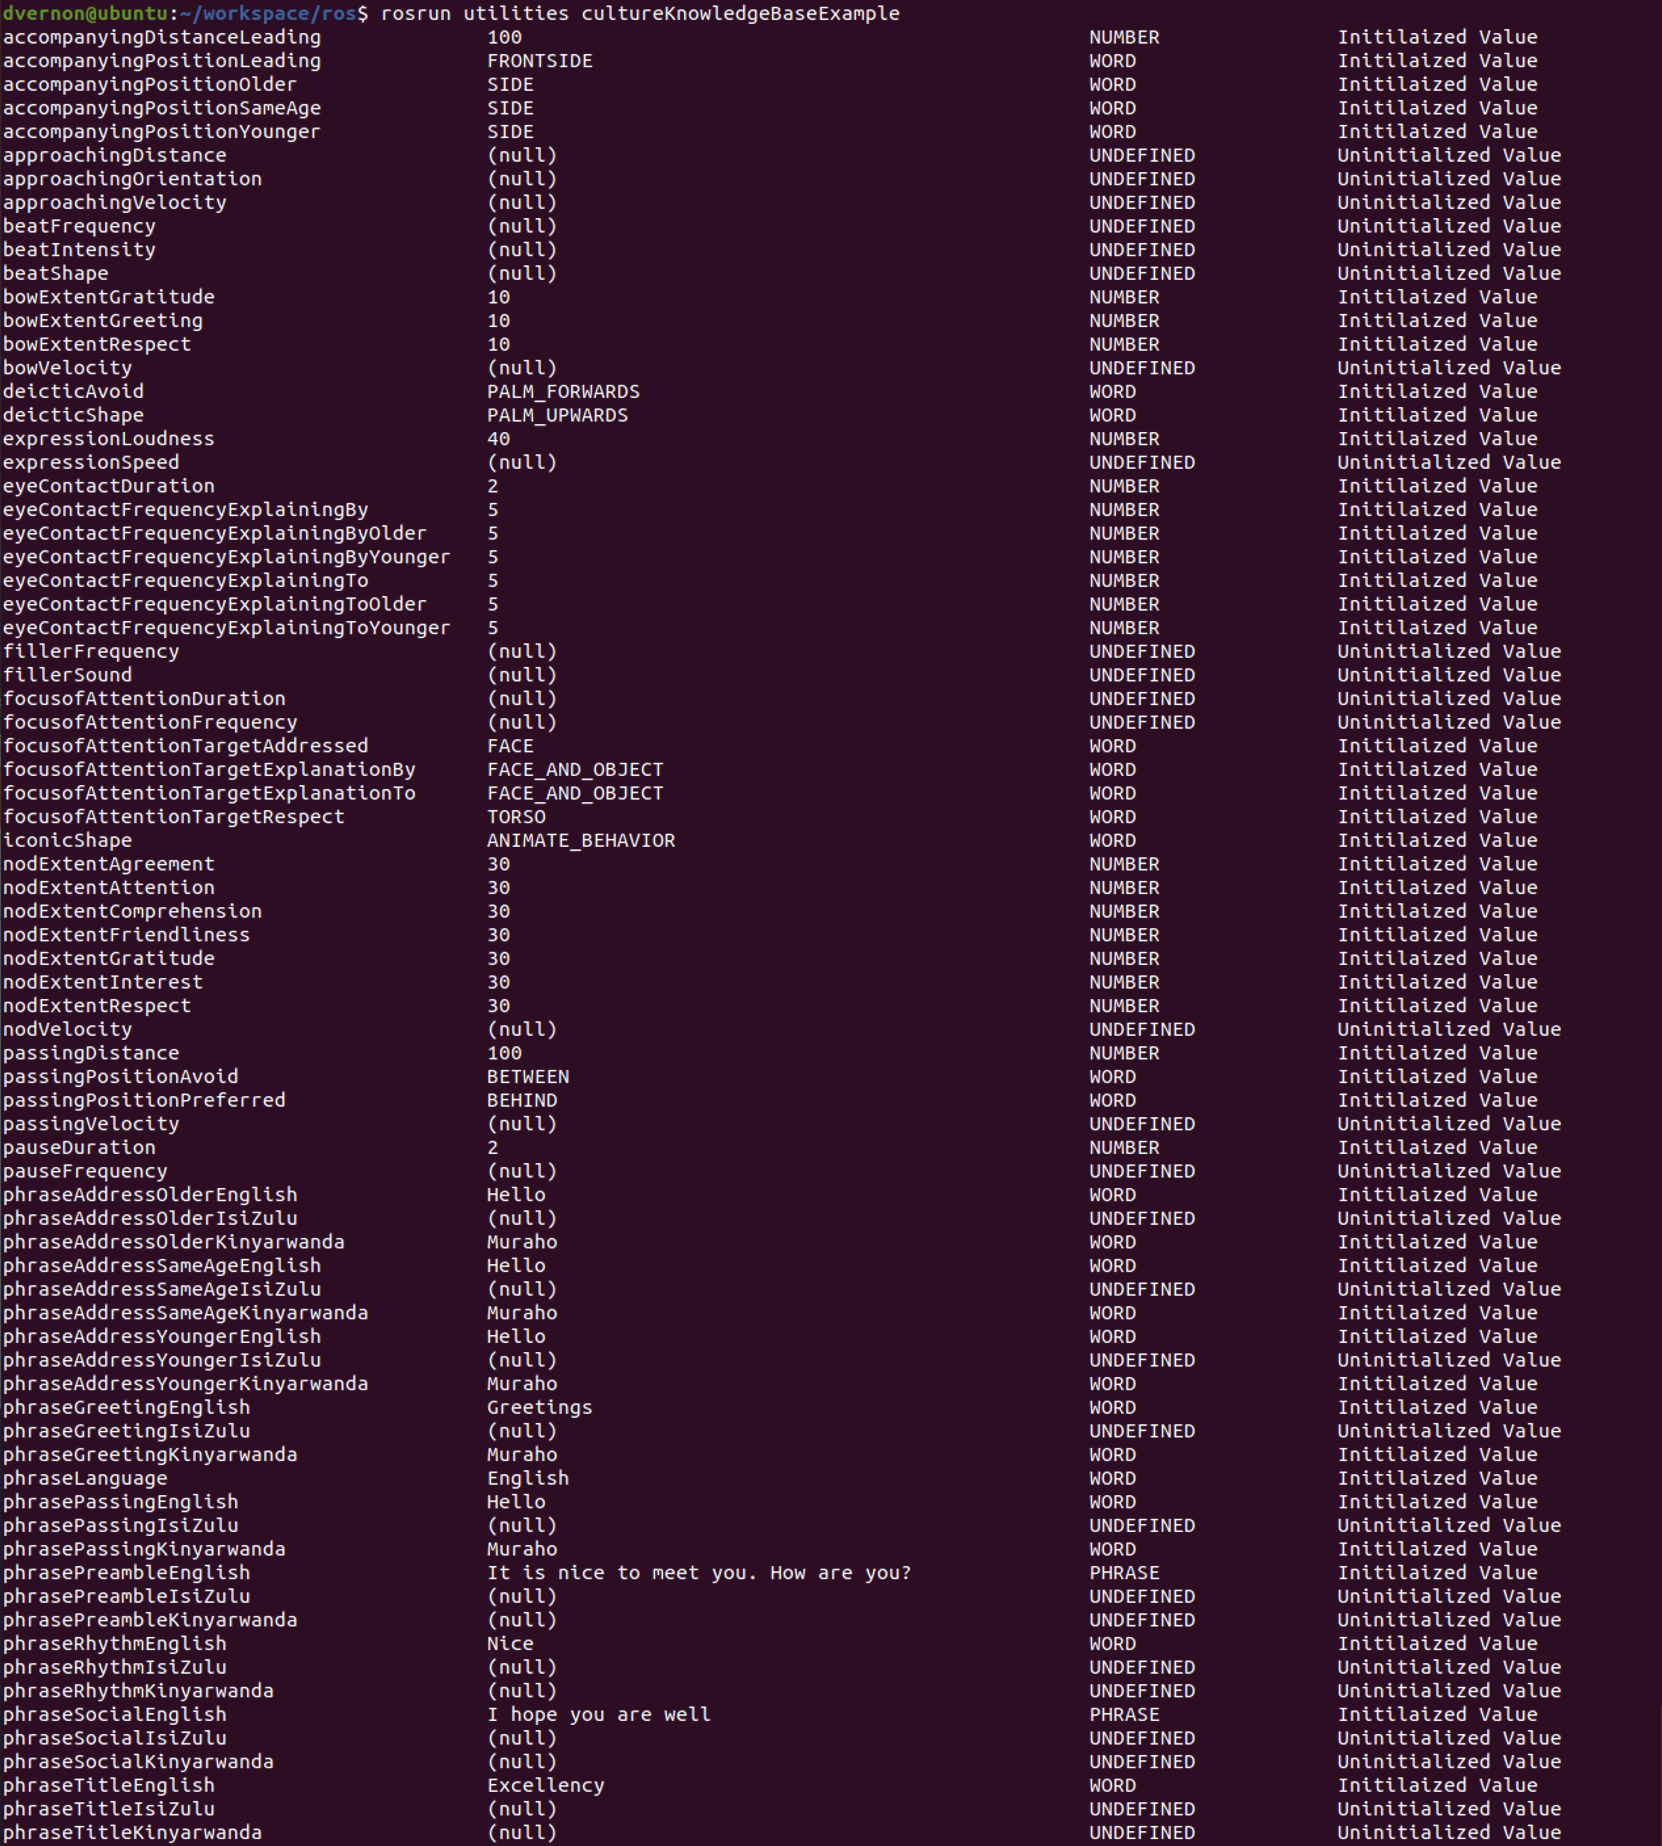
\includegraphics[width=155mm,angle=0]{screenshot1.png}\\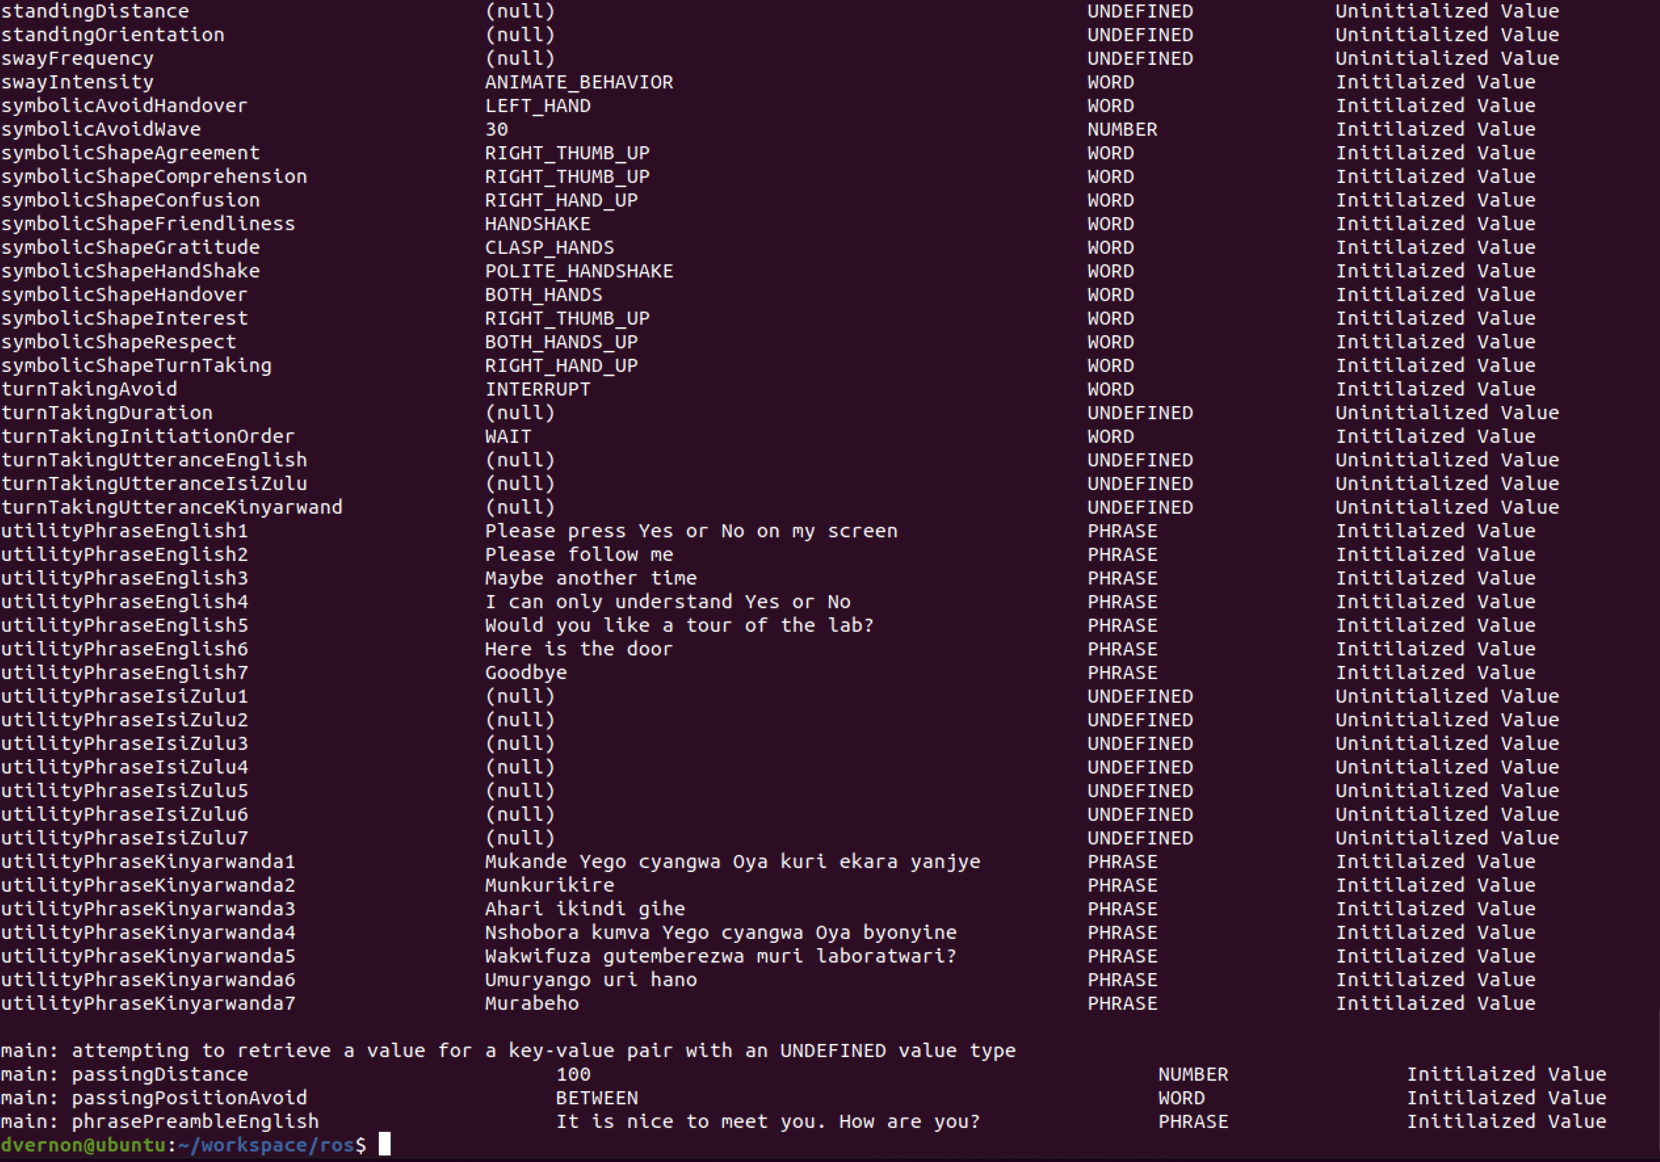
\includegraphics[width=155mm,angle=0]{screenshot2.png}
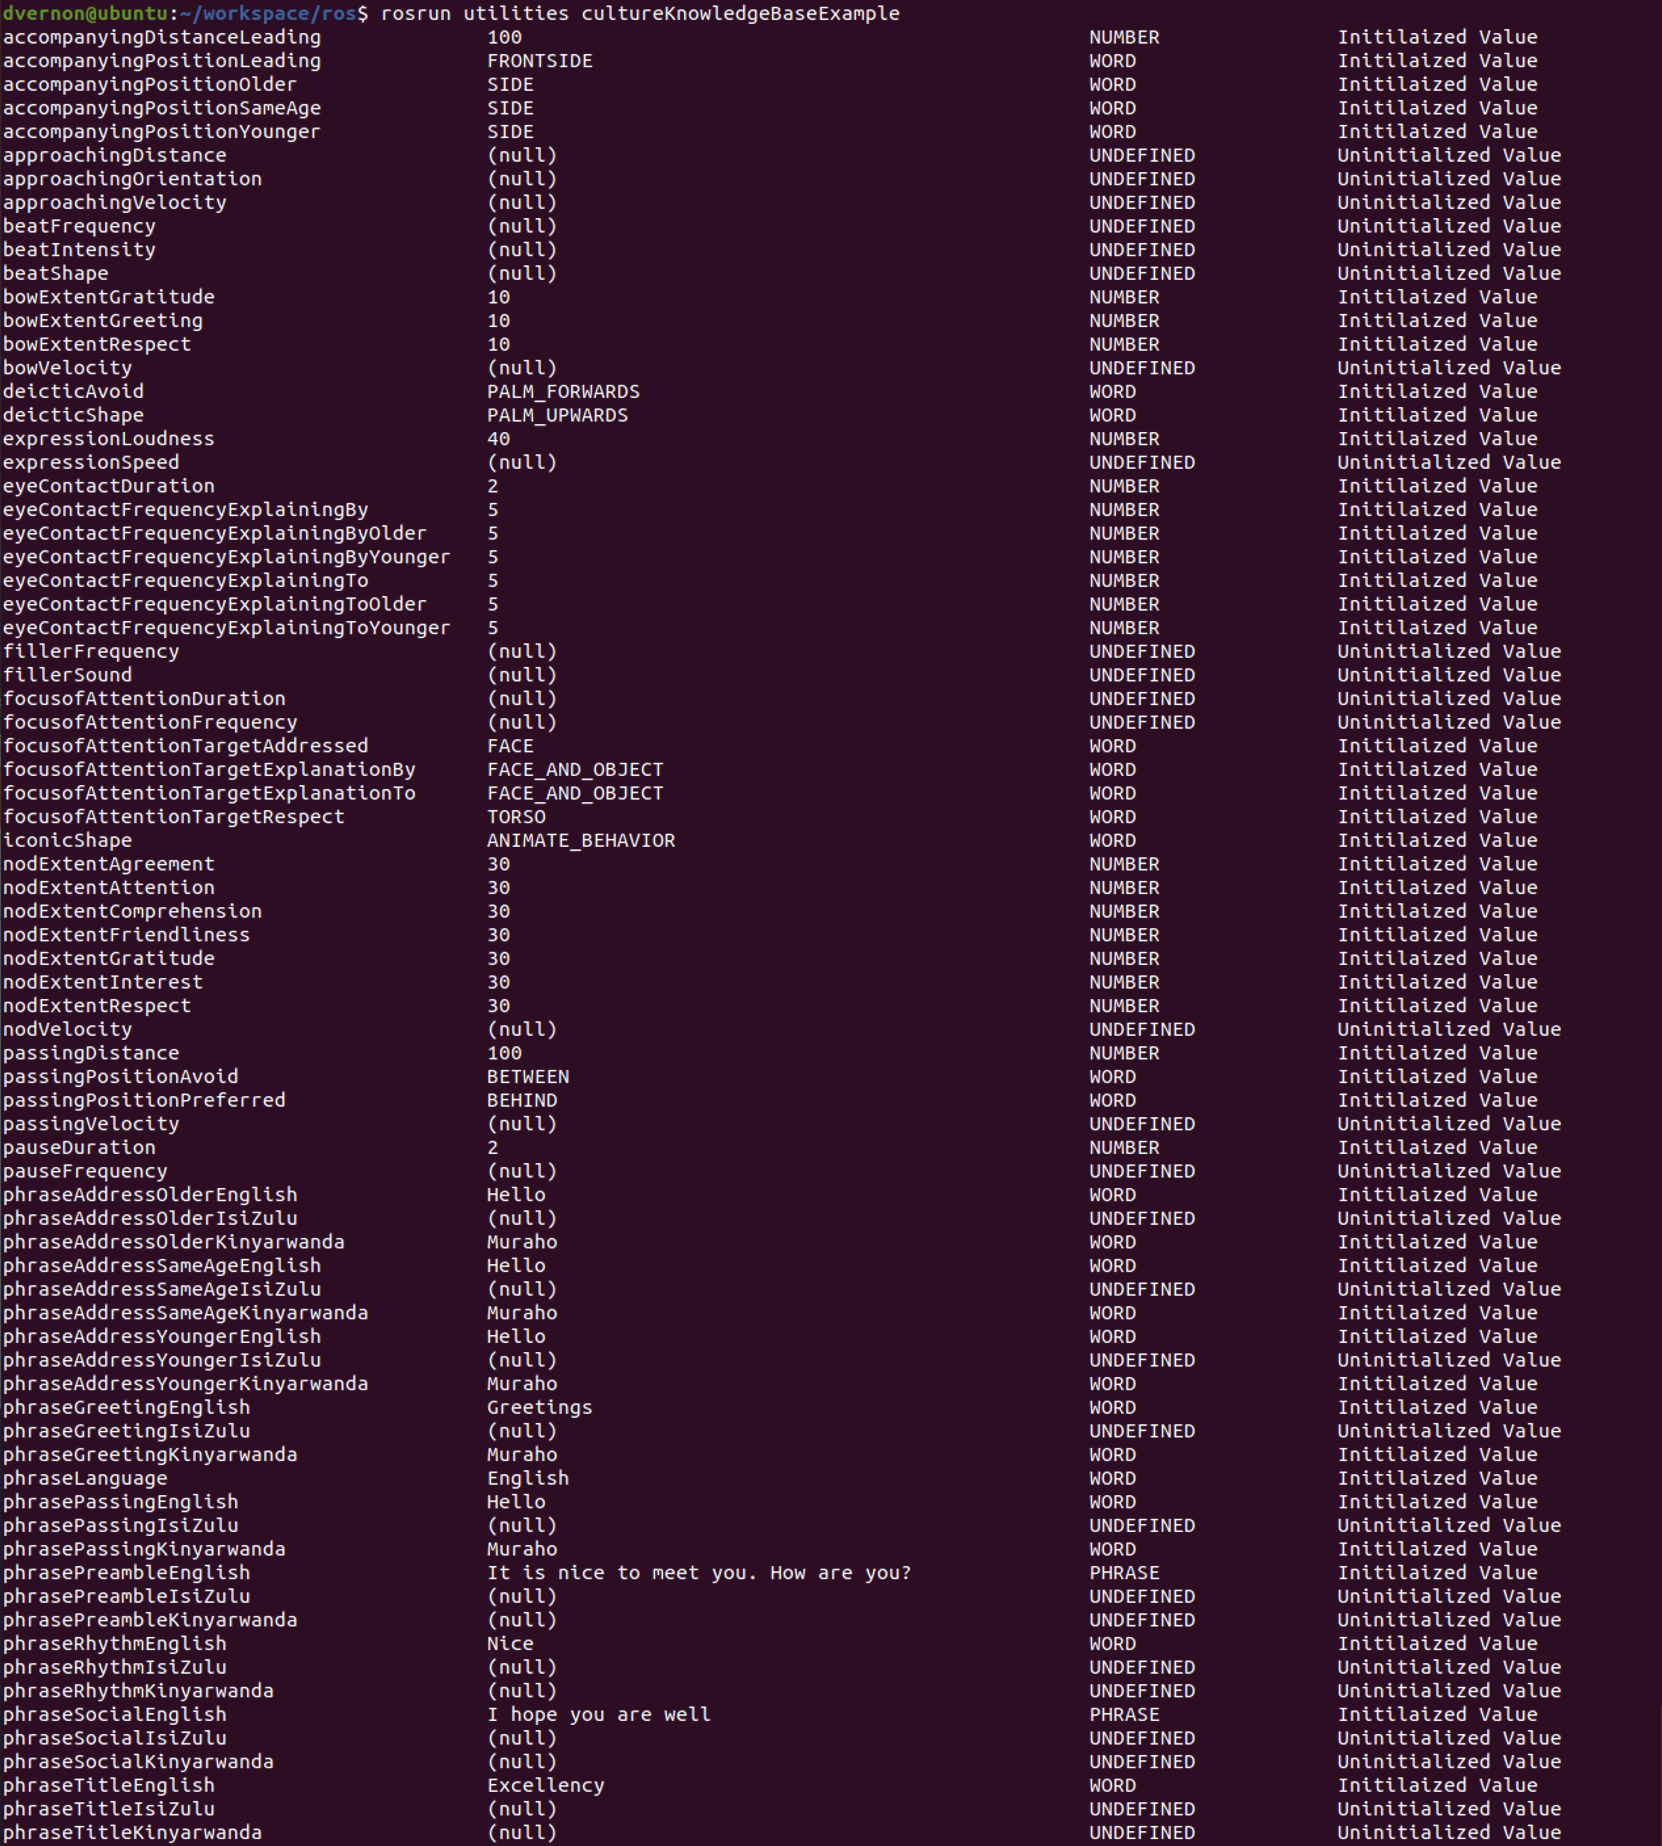
\includegraphics[width=125mm,angle=0]{screenshot1.png}\\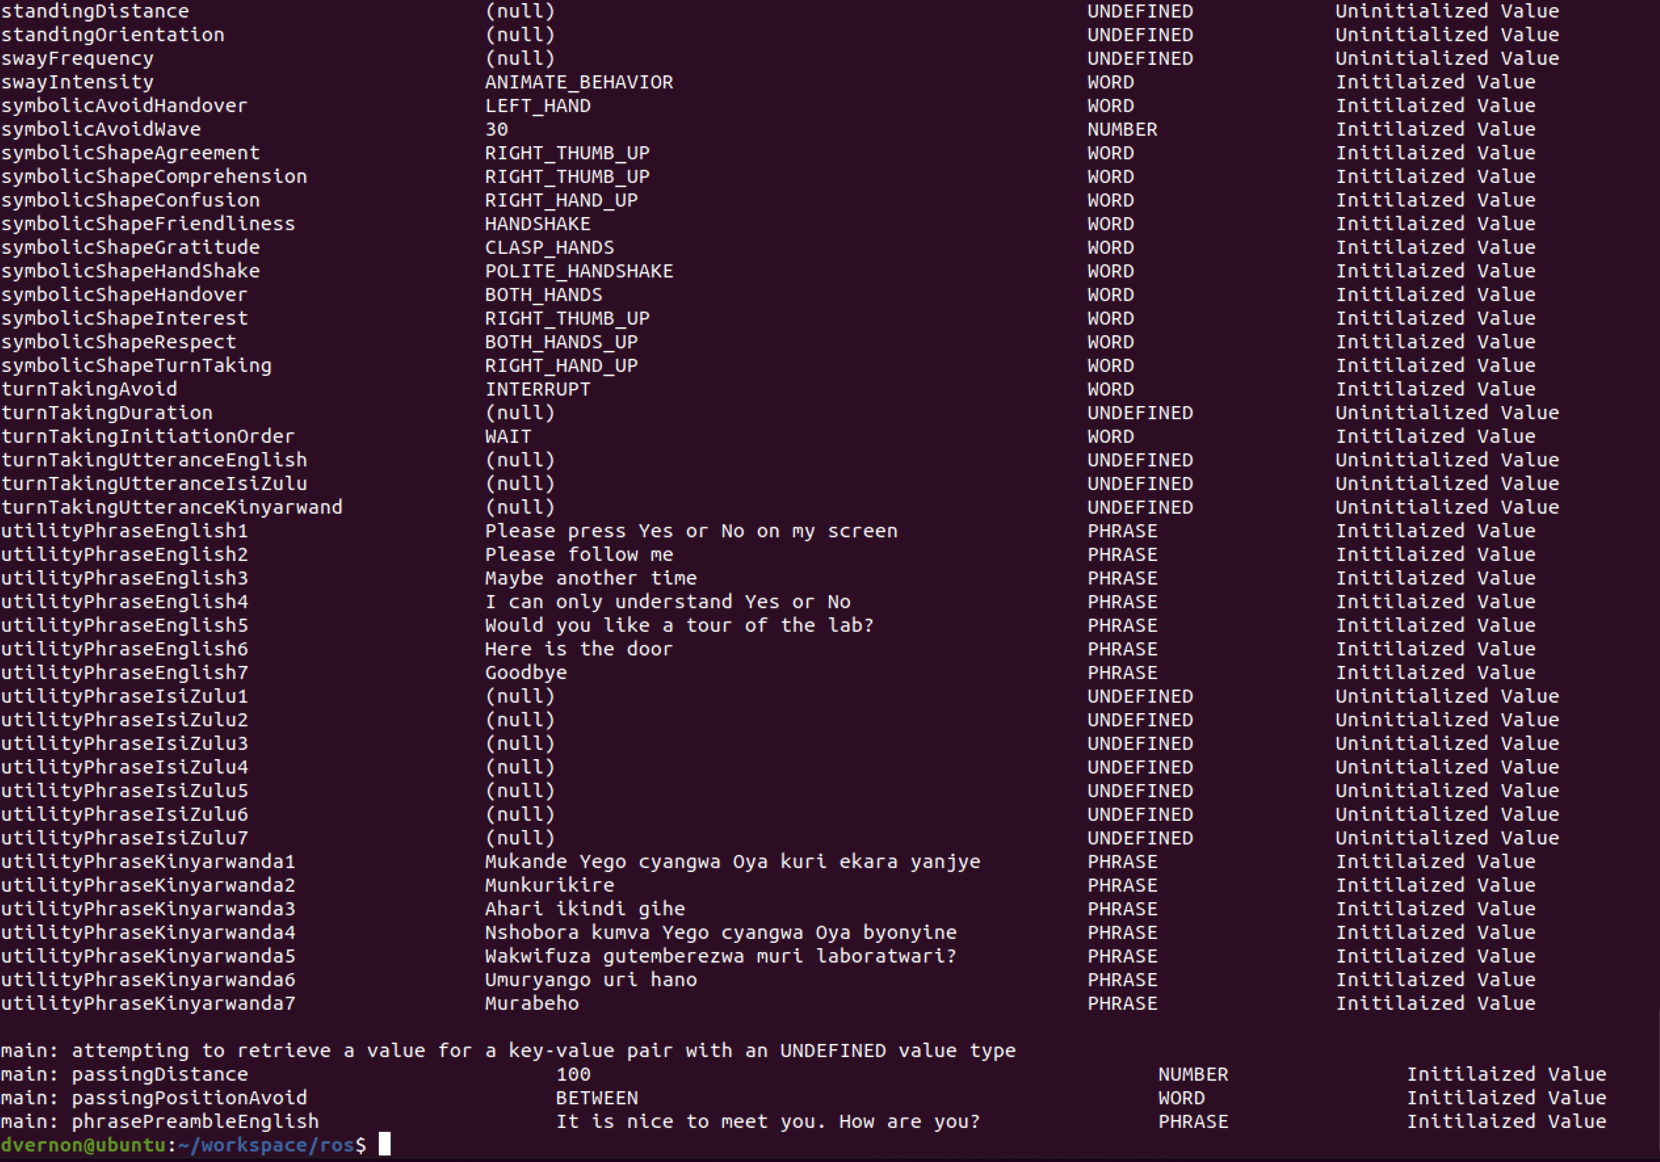
\includegraphics[width=125mm,angle=0]{screenshot2.png}
\end{center}
%\vspace{-5mm}
\caption{Screenshot of  the output of running the example  application.}
\label{fig:screenshot}       
\end{figure}



\newpage
\begin{appendices}
%###############################################################################

%===============================================================
\section{The CultureKnowledgeBase Class}
%===============================================================
\label{appendix:helper_class}  

Note: documentation comments for the private methods have been removed due to space constraints but are retained in the source file.

\lstdefinestyle{withoutNumbering}{
    backgroundcolor=\color{backcolour},   
    commentstyle=\color{codegreen},
    keywordstyle=\color{magenta},
    stringstyle=\color{codepurple},
    %%basicstyle=\ttfamily\small,
    basicstyle=\ttfamily\tiny,
    breakatwhitespace=false,         
    breaklines=true,                 
    captionpos=b,                    
    keepspaces=true,                 
    showspaces=false,                
    showstringspaces=false,
    showtabs=false,                  
    tabsize=2
}
\begin{lstlisting}[style=withoutNumbering, language=bash]

#define NUMBER_OF_CONFIGURATION_KEYS   3
#define NUMBER_OF_VALUE_TYPES          4

/* constant definitions for valueType flag to identify which element of the union is to be used */

#define UNDEFINED 0 // value hasn't been initialized
#define NUMBER    1 // value is integer
#define WORD      2 // value is alphanumeric but just one word
#define PHRASE    3 // value is alphanumeric but several words

typedef char Keyword[KEY_LENGTH];

typedef struct {
   char knowledgeBase[MAX_FILENAME_LENGTH];
   char valueTypes[MAX_FILENAME_LENGTH];
   bool verboseMode;
} ConfigurationDataType;

typedef  struct {
    char *key;
    union {
        int   integerValue;
        char* alphanumericValue;  
    };
    int valueType;
    bool initialized;
} KeyValueType;

typedef struct node *NodeType;

typedef struct node {
            KeyValueType keyValue;
            NodeType left, right;
         } Node;

typedef NodeType BinaryTreeType;

typedef BinaryTreeType WindowType;

class CultureKnowledgeBase {
public:
   CultureKnowledgeBase();
   ~CultureKnowledgeBase();
   bool                  getValue(char *key, KeyValueType *keyValue);   
   void                  print_to_screen();                                   

private:

   /* data members */
   KeyValueType          keyValue;
   BinaryTreeType        tree = NULL; 
   ConfigurationDataType configurationData;
   char                  configuration_filename[MAX_STRING_LENGTH] = "cultureKnowledgeBaseConfiguration.ini";
   
   /* methods */
   void                  assign_key_attributes(KeyValueType *keyValue, char key[],  int valueType, bool operational);   
   void                  assign_key_value(KeyValueType *keyValue, int integerValue, bool operational);   
   void                  assign_key_value(KeyValueType *keyValue, char *alphanumericValue, bool operational);     
   KeyValueType          delete_min(BinaryTreeType *tree);      
   BinaryTreeType        *delete_element(KeyValueType keyValue, BinaryTreeType *tree);  
   bool                  exists(char *key);   
   bool                  exists(KeyValueType keyValue, BinaryTreeType *tree);  
   int                   height();    
   int                   height(BinaryTreeType tree, int n);  
   int                   getValueType(char *key);  
   bool                  getValue(char *key, KeyValueType *keyValue, BinaryTreeType *tree);   
   void                  initialize(BinaryTreeType *tree);  
   BinaryTreeType        *insert(KeyValueType keyValue, BinaryTreeType *tree, bool update);   
   int                   inorder_print_to_screen(BinaryTreeType tree, int n);  
   int                   inorder_print_to_file(BinaryTreeType tree, int n, FILE *fp_out); 
   int                   postorder_delete_nodes(BinaryTreeType tree); 
   int                   print_to_file(FILE *fp_out);  
   int                   print_to_file(BinaryTreeType tree, FILE *fp_out);  
   int                   print_to_screen(BinaryTreeType tree);      
   int                   size(BinaryTreeType tree);   
   void                  readConfigurationData();  
   void                  readKnowledgeBase();   
   void                  readKnowledgeBaseValueTypes();    
   int                   size(); 
   int                   total_number_of_probes();    
   int                   total_number_of_probes(BinaryTreeType tree, int n);        
};




\end{lstlisting}

 \end{appendices}
%###############################################################################



\newpage
\bibliographystyle{unsrt}
%================================================================
\bibliography{cognitive_systems.bib}                                     % REPLACE with correct filename
\addcontentsline{toc}{section}{References}

 

\pagebreak
\section*{Principal Contributors}
%===============================================================
\label{contributors}
\addcontentsline{toc}{section}{Principal Contributors}
The main authors of this deliverable are as follows (in alphabetical order).
\blank
~
\blank
Eyerusalem Birhan, Carnegie Mellon University Africa.\\    
Muhirwa Richard, Carnegie Mellon University Africa.\\   
David Vernon, Carnegie Mellon University Africa.\\   
  

\newpage
\section*{Document History}
%================================================================
\addcontentsline{toc}{section}{Document History}
\label{document_history}

\begin{description}

\item [Version 1.0]~\\
First version created by moving and reorganizing Section 2 Representation of Cultural Knowledge and Section 3.2 Action and Cultural Parameter Values from Deliverable D1.2. \\
David Vernon.\\
30 December 2024.   \\                                           

\item [Version 1.1]~\\
Changed ontology category from Words to Expression.\\
Introduced an extended ontology tree  in which there is at least one leaf node for each consensus answer; see  Fig. \ref{fig:knowledge_ontology2} .\\
Added Tables \ref{table:key-value_questions_spatial} - \ref{table:key-value_pairs3}.\\
Added Section \ref{section:implementation} Implementation.\\
David Vernon.\\
25 February 2025. \\   

\item [Version 1.2]~\\
Added launch subdirectory and launch file to the directory structure in Figure \ref{fig:directory_structure_utilities}.\\
David Vernon.\\
28 February 2025. \\ 

\item [Version 1.3]~\\
Changed {\tt \small cultureKnowledgeBase.dat} and {\tt \small cultureKnowledgeBaseValueTypes.dat} to {\tt \small cultureKnowledgeBaseInput.dat} and {\tt \small cultureKnowledgeBaseInput.dat} to be compliant with the software engineering standards.\\
David Vernon.\\
3 March 2025. \\ 


\item [Version 1.4]~\\
Changed {\tt \small cultureKnowledgeBase.dat} and {\tt \small cultureKnowledgeBaseValueTypes.dat} to {\tt \small cultureKnowledgeBaseInput.dat} and {\tt \small cultureKnowledgeBaseInput.dat} to be compliant with the software engineering standards.\\
David Vernon.\\
3 March 2025. \\ 

\item [Version 1.5]~\\
Removed  the {\small \tt utilities} sub-directory since the C++ helper classes will be integrated directly in the software for the {\small \tt behaviorController} node and not be made available independently.\\
Extended the ontology and added new keys to allow for phrases and utterances in English, isiZulu, and Kinyarwanda.\\
David Vernon.\\
11 March 2025.   \\   

\item [Version 1.6]~\\
Adjusted tables and text to ensure they stay within the set margins.\\
David Vernon.\\
25 March 2025.   \\  

\item [Version 2.0]~\\
Changed all keys to camel case.\\
Added utility verbal interaction phrases.\\
David Vernon.\\
15 April 2025.   \\  

\item [Version 2.1]~\\
Changed instances of {\small \tt expressionPhrase*} keys to {\small \tt phrase*} keys in Table \ref{table:key-value_questions_verbal} to be consistent with keys in Table \ref{table:key-value_pairs2}.\\
David Vernon.\\
1 May 2025.   \\  

\end{description}


\end{document}
